\documentclass[11pt]{report} % Define la clase de documento como 'report' con tamaño de fuente 11pt
\usepackage{geometry} % Paquete para personalizar los márgenes del documento
\usepackage[utf8]{inputenc} % Permite la introducción de caracteres UTF-8
\usepackage[greek, spanish, es-tabla]{babel} % Establece idiomas para el documento
\usepackage[bottom]{footmisc} % Coloca las notas al pie en la parte inferior de la página
\usepackage[tt]{titlepic} % Permite incluir una imagen en la página de título con una fuente mono-spaced
\usepackage{url} % Permite la inserción de URL en el documento
\usepackage{xurl} % Mejora el manejo de URL en el documento
\usepackage{graphicx} % Permite la inclusión de gráficos en el documento
\usepackage{makeidx} % Facilita la creación de índices
\usepackage{enumerate} % Permite la personalización de listas enumeradas
\usepackage{lastpage} % Proporciona una referencia a la última página del documento
\usepackage{fancyhdr, ragged2e} % Personaliza los encabezados y pies de página
\usepackage{eurosym} % Permite la inserción del símbolo de euro
\usepackage{float} % Mejora el posicionamiento de los elementos flotantes en el documento
\usepackage{titlesec} % Facilita la personalización de títulos de secciones
\usepackage{hyperref} % Permite la creación de enlaces hipertexto
\usepackage{nameref} % Permite hacer referencia al nombre de secciones
\usepackage{enumitem} % Permite personalizar listas
\usepackage{booktabs} % Mejora la apariencia de las tablas
\usepackage[table]{xcolor} % Permite el uso de colores en tablas
\usepackage{multirow} % Permite combinar celdas en tablas
\usepackage{amsmath} % Proporciona funciones matemáticas avanzadas
\usepackage{tikz} % Permite la creación de gráficos vectoriales
\usetikzlibrary{shadings} % Carga la librería para degradados en los gráficos de TikZ
\usepackage[nameinlink]{cleveref} % Facilita las referencias cruzadas con nombres
\usepackage{listings} % Permite la inclusión de código fuente en el documento
\usepackage{microtype} % Para mejor formato de texto
\usepackage[normalem]{ulem} % Para subrayado con color
\usepackage{palatino} %La fuente Libertine también se ve bien
\usepackage[T1]{fontenc}


% Ajustes de los márgenes de la página
\addtolength{\oddsidemargin}{-.8in}
\addtolength{\evensidemargin}{-.8in}
\addtolength{\textwidth}{1.45in}
\addtolength{\topmargin}{-.1in}
\addtolength{\textheight}{1.25in}


\graphicspath{{figures/}} % Directorio donde se encuentran los archivos de imágenes
\pagestyle{fancy} % Estilo de página personalizado
\renewcommand{\chaptermark}[1]{\markboth{\scriptsize\MakeUppercase{#1}}{}} % Configuración del marcado de capítulos
\renewcommand{\sectionmark}[1]{\markright{\tiny\MakeUppercase{#1}}{}} % Configuración del marcado de secciones


% Configuración del pie de página
\fancypagestyle{plain}{
    \renewcommand{\headrulewidth}{0pt} 
    \fancyfoot[L]{\raisebox{-0.6cm}{\includegraphics[height=1cm]{figures/EscudoUniovi.jpg}}}
    \fancyfoot[C]{\scriptsize BidMon Universe. Plataforma de coleccionismo de cartas digitales. \\ Trabajo Fin de Grado Ingeniería Informática del Software \textbar{} Versión 0.1 \\ Paula Suárez Prieto}
    \fancyfoot[R]{\thepage\ de \pageref{LastPage}}
    \renewcommand{\footrulewidth}{0.4pt}
}




%Evita warnings de cabecera
\setlength{\headheight}{15pt}
\setcounter{secnumdepth}{4}

%Esto es para poder ponerle un formato bien hecho a los \paragraph{}
\titleformat{\paragraph}
{\normalfont\normalsize\bfseries}{\theparagraph}{1em}{}
\titlespacing*{\paragraph}
{0pt}{3.25ex plus 1ex minus .2ex}{1.5ex plus .2ex}

%Y esto para para ponerselo a los \subparagraph{}
\titleformat{\subparagraph}
{\normalfont\normalsize\bfseries}{\theparagraph}{1em}{}
\titlespacing*{\subparagraph}
{0pt}{1ex plus 1ex minus .2ex}{1.5ex plus .2ex}

% Configuración para permitir la numeración hasta el quinto nivel
\setcounter{secnumdepth}{5}

% Crear un nuevo contador para subsubsubsection que se reinicia con cada subsubsection
\newcounter{subsubsubsection}[subsubsection]

% Formatear el contador para que se muestre como subsubsection.subsubsubsection
\renewcommand{\thesubsubsubsection}{\thesubsubsection.\arabic{subsubsubsection}}

\newcommand{\subsubsubsection}[1]{%
  \refstepcounter{subsubsubsection}
  \paragraph{#1}\vspace{3mm}
}


% Formato para el título de subsubsubsection
\titleformat{\paragraph}
  {\normalfont\normalsize\bfseries\itshape}{\thesubsubsubsection}{1em}{}
\titlespacing*{\paragraph}
  {0pt}{3.25ex plus 1ex minus .2ex}{-1ex plus .2ex}


% Colores usados en las tablas
\definecolor{headercolor}{rgb}{.871,  .918,  .965}
\definecolor{rowcolor}{rgb}{.949,  .949,  .949}
\definecolor{darkgreen}{rgb}{0.525, 0.655, 0.537}
\definecolor{lightgreen}{rgb}{0.824, 0.890, 0.784}
\definecolor{linkColor}{HTML}{086554}


% Configuración de los estilos del capítulo
\titleformat{\chapter}[display]
  {\normalfont\huge\bfseries\raggedright}
  {\color{darkgreen}\chaptertitlename\ \thechapter}{20pt}{\Huge\color{black}\raggedright}

% Estilos de los enlaces 
\hypersetup{
    colorlinks = true, % Colores en los enlaces 
    linkcolor = linkColor, % Color de los enlaces internos
    filecolor = linkColor, % Color de los enlaces a archivos
    urlcolor = linkColor, % Color de los enlaces externos
    citecolor = linkColor
}

% Comando para subrayar enlaces
\newcommand{\coloredUnderline}[1]{\bgroup\markoverwith{\textcolor{linkColor}{\rule[-0.5ex]{2pt}{0.4pt}}}\ULon{#1}}


\phantomsection
\makeindex

\begin{document}
\selectlanguage{spanish} 


\hypersetup{pageanchor=false}

% ----- Portada -----
\begin{titlepage}
	\centering
	\includegraphics[width=0.2\textwidth]{EscudoUniovi}
	\hspace{3 cm}
	\includegraphics[width=0.3\textwidth]{EscudoEscuela}
	\par\vspace{1cm}
	
	\vspace{1.5cm}
	{\huge\bfseries BidMon Universe \\ Plataforma de coleccionismo de cartas digitales\par}
	\vspace{2cm}
	{\large \textbf{GRADO EN INGENIERÍA INFORMÁTICA DEL SOFTWARE} \par}
	\vspace{1cm}
	{\scshape\Large Trabajo Fin de Grado\par}
   	
  \vspace{2cm}
	\textbf{AUTOR}\par
	Paula Suárez Prieto \\
	\vspace{1.5cm}
	\textbf{TUTOR}\par
	Hugo Lebredo Buján
	\vfill
	
	{\large Julio 2024 \par}
\end{titlepage}
% ----- Fin Portada -----

% ----- Página de copyright -----
\newpage
\pagestyle{plain}
Copyright (C) 2020 \textbf{ELENA ALLEGUE GONZÁLEZ, JOSÉ MANUEL REDONDO LÓPEZ} \\
Teaching Innovation Project: PINN-19-A-029 (University of Oviedo)\\
This work has been published in \cite{RedondoPlantillasRG19} \cite{RedondoUCO20}\\
\\
Esta versión de la plantilla para Trabajos de Fin de Grado ha sido posible gracias a la donación de la ex-alumna Elena Allegue González de su documentación de Trabajo de Fin de Grado, que ha servido como base para elaborar esta versión. Aquí podréis encontrar todos los títulos y subtítulos de las secciones, pero las explicaciones se mantendrán en la versión \textit{Word} de la plantilla (se proporciona una versión PDF de la misma para facilitar el acceso a las mismas). No obstante, del trabajo de Elena se han conservado ejemplos de como hacer elementos clave como imágenes, tablas, etc.

Desarrollar una versión \textit{Latex} de la plantilla desde cero es una trabajo bastante largo, pero gracias al trabajo de Elena se ha podido equiparar esta versión con las de \textit{Word} mucho más rápidamente.
% ----- Fin Página de copyright -----

%\newpage
\pagestyle{fancy}
\chapter*{Agradecimientos}

\pagestyle{fancy}

% Redefine el comando \chaptermark para personalizar el encabezado de los capítulos
\renewcommand{\chaptermark}[1]{ 
    % Marca ambos encabezados izquierdo y derecho con el título del capítulo
    \markboth{\scriptsize\MakeUppercase{#1}}{} 
}

% Redefine el comando \sectionmark para personalizar el encabezado de las secciones
\renewcommand{\sectionmark}[1]{ 
    % Marca el encabezado derecho con el título de la sección
    \markright{\tiny\MakeUppercase{#1}}{} 
}


%\Configuración del pie de página

\fancyfoot{}
\fancyfoot[L]{\raisebox{-0.6cm}{\includegraphics[height=1cm]{figures/EscudoUniovi.jpg}}}

\fancyfoot[R] {\thepage\ de \pageref{LastPage}}
\fancyfoot[C]{\scriptsize BidMon Universe. Plataforma de coleccionismo de cartas digitales. \\ Trabajo Fin de Grado Ingeniería Informática del Software \textbar{} Versión 0.1 \\ Paula Suárez Prieto   }
\setlength{\footskip}{32.93277pt}
\renewcommand{\footrulewidth}{0.4pt}
\pagenumbering{arabic}


\pagestyle{plain}


\setcounter{tocdepth}{2}
\setcounter{secnumdepth}{4}

% ----- Página de Lista de contenidos -----
\pagestyle{plain}
{
  \hypersetup{hidelinks}
  \renewcommand{\thispagestyle}[1]{}
  \tableofcontents
}
\clearpage

% ----- Página de Lista de figuras -----
\newpage
{
  \hypersetup{hidelinks}
  \renewcommand{\thispagestyle}[1]{}
  \listoffigures
}
\clearpage

% ----- Página de Lista de tablas -----
\newpage
{
  \hypersetup{hidelinks}
  \renewcommand{\thispagestyle}[1]{}
  \listoftables
}
\clearpage

\newpage
\hypersetup{pageanchor=true}

\newpage


\newpage
\thispagestyle{empty}
\chapter{Introducción}
\noindent\begin{tikzpicture}
% Definir el degradado
\shade[left color=darkgreen, right color=lightgreen] (0,0) rectangle (\textwidth-1pt,0.2);

\end{tikzpicture}
\section{Resumen}
El coleccionismo de cartas es una actividad que ha ganado popularidad en los últimos años, especialmente con la llegada de las cartas de Pokémon.
Las subastas de cartas son una forma de adquirir cartas raras y valiosas, pero pueden ser complicadas de seguir y participar.
En este proyecto se propone el desarrollo de una aplicación web que permita a los usuarios seguir y participar en subastas de cartas de Pokémon de forma sencilla y segura.


\section{Palabras Clave}
Coleccionismo, subastas, cartas, Pokémon


\section{\textit{Abstract}}
Card collecting is an activity that has gained popularity in recent years, especially with the arrival of Pokémon cards.
Card auctions are a way to acquire rare and valuable cards, but they can be difficult to follow and participate in.
This project proposes the development of a web application that allows users to follow and participate in Pokémon card auctions in a simple and secure way.



\section{\textit{Keywords}}
Collecting, auctions, cards, Pokemon

\newpage
\pagestyle{fancy}

%\newpage
\chapter{PLANIFICACIÓN DEL SISTEMA DE INFORMACIÓN}

\noindent\begin{tikzpicture}
% Definir el degradado
\shade[left color=darkgreen, right color=lightgreen] (0,0) rectangle (\textwidth-1pt,0.2);

\end{tikzpicture}
\newpage

\section{INICIO DEL PLAN DE SISTEMAS DE INFORMACIÓN}
\subsection{Análisis de la Necesidad del Plan de Sistemas de Información}
Con la tecnología, la forma en la que nos relacionamos con nuestros pasatiempos ha cambiado. La popularidad de plataformas como EA Sports FC y su modo Ultimate Team\cite{artsEASPORTSFC2023}, 
deja en evidencia que el mercado de coleccionismo digital está en pleno crecimiento \cite{sanmartin000MillonesDolares2021}. 
Sin embargo, aún existe un nicho de mercado específico por explorar: una plataforma dedicada exclusivamente al coleccionismo de cartas digitales.

BidMon Universe trata de dar respuesta a esta necesidad, ofreciendo a los coleccionistas digitales una forma segura e innovadora de comprar y vender activos digitales mediante un sistema de pujas ciego.

El Plan de Sistemas de Información para este proyecto se aborda desde una perspectiva que considera tanto la arquitectura técnica como la experiencia del usuario final. 
De esta manera se establece un marco de trabajo que garantiza que, además de cumplir con las expectativas del mercado actual, el proyecto proporciona características y experiencias novedosas 
que enriquecen la dinámica del coleccionismo digital.

\subsection{Identificación del Alcance del Plan de Sistemas de Información} \hypertarget{sec:2_identificacion_alcance_PSI}{}
La aplicación web a desarrollar deberá de proporcionar al usuario final las siguientes funcionalidades de alto nivel:
\begin{itemize}
    \item Todo usuario final puede acceder a la aplicación web y consultar información genérica sobre la misma.
    \begin{itemize}
        \item Información sobre el servicio que se ofrece.
        \item Información sobre el equipo de desarrollo.
    \end{itemize}
    \item Cualquier usuario, mayor de 18 años, podrá crear una cuenta de usuario en la aplicación.
    \item Cualquier usuario registrado en la aplicación puede iniciar sesión en esta.
    \item Los usuarios autenticados tendrán una colección de cartas digitales que podrán consultar.
    \item Los usuarios autenticados pueden recargar el saldo de su cuenta.
    \item Los usuarios autenticados tendrán acceso a un catálogo de sobres de cartas que podrán adquirir si cuentan con saldo suficiente.
    \item Los usuarios autenticados podrán realizar subastas y pujas ciegas sobre las cartas.
    \item Los usuarios autenticados podrán consultar el histórico de transacciones realizadas.
    \item Los usuarios autenticados podrán modificar su perfil.
    \item Los usuarios autenticados podrán consultar el perfil de las personas que están subastando cartas. Se mostrará la siguiente información:
    \begin{itemize}
        \item Cartas destacadas del usuario. Por ejemplo, si este posee una carta rara podrá seleccionarla como destacada para mostrarla en su perfil.
        \item Número de pujas en las que ha participado.
        \item Número de subastas que ha realizado.
        \item Subastas activas.
    \end{itemize}
    \item Un usuario con rol de administrador podrá acceder al histórico de subastas y cancelar las que considere fraudulentas, el sistema notificará al usuario que la ha iniciado.
\end{itemize}

En base a estas funcionalidades se extraen los siguientes \textbf{objetivos estratégicos} a lograr para alcanzar el éxito del proyecto:

\begin{itemize}
    \item Implementar un sistema de autenticación de usuarios.
    \item Implementar un sistema de venta de cartas.
    \item Implementar un sistema de subastas ciegas que permita a los usuarios comprar y vender cartas.
    \item Implememntar un sistema de gestión de subastas por parte de un usuario autenticado.
    \item Implememntar un sistema de gestión de subastas por parte de un usuario administrador.
    \item Implementar un sistema de notificaciones que informe a los usuarios sobre el estado de las subastas en las que participan.
    \item Interfaz intuitiva que permita al usuario realizar consultas sobre el estado de las pujas y subastas, además de visualizar la colección de cartas adquirida.
\end{itemize}

\subsection{Determinación de Responsables}
A continuación, se detallan las personas que participan en el proyecto junto con sus funciones.
\begin{itemize}
    \item El tutor del trabajo se encargará de la supervisión del proyecto.
    \item El alumno se encargará del desarrollo del proyecto y documentación de este. 
\end{itemize}

\newpage
\section{DEFINICIÓN Y ORGANIZACIÓN DEL PLAN DE SISTEMAS DE INFORMACIÓN}
 

\subsection{Especificación del Ámbito y Alcance} 
La plataforma a desarrollar, BidMon Universe, tiene como objetivo principal permitir al usuario coleccionar activos digitales, en este caso, cartas. 
Estas se pueden obtener mediante una compra directa a la aplicación o por medio de subastas.

La aplicación contará con una moneda virtual que permitirá a los usuarios adquirir cartas y participar en subastas. Los usuarios podrán recargar su saldo mediante una pasarela de pago.
Un usuario autenticado tendrá la posibilidad de comprar cartas y si desea venderlas, podrá hacerlo mediante subastas ciegas. 
El usuario tiene una colección privada de cartas que podrá consultar en cualquier momento. Tiene la posibilidad de marcar una carta como destacada para mostrarla en su perfil.

Las subastas funcionarán de la siguiente manera: un usuario podrá subastar una carta y otros usuarios podrán pujar por ella.
El sistema de subastas será ciego, es decir, los usuarios no podrán ver las pujas de los demás. 
El usuario que haya realizado la puja más alta al finalizar la subasta será el ganador y se le descontará el importe de su puja del saldo de su cuenta.
El usuario que vende la carta tiene posibilidad de personalizar los términos de la subasta, como la duración de la misma o el precio de salida. Además, podrá cancelar la subasta en cualquier momento.

La plataforma contará con un sistema de notificaciones que informará a los usuarios sobre el estado de las subastas en las que participan o han iniciado.

Se llevará un registro de todas las transacciones realizadas en la plataforma para garantizar la trazabilidad y transparencia de las operaciones. 
Se registrarán tanto las compras directas como las subastas y pujas realizadas. Las cartas adquiridas tendrán un historial de transacciones asociado.

Todos los usuarios tendrán acceso a un panel de control donde podrán consultar el histórico de transacciones realizadas y modificar su perfil.

Los administradores del sistema tendrán acceso a un panel de control donde podrán consultar el histórico de subastas y cancelar aquellas que consideren fraudulentas. 
También podrán consultar el histórico de transacciones realizadas en la plataforma.


Debido a la naturaleza dle proyecto, se han establecido las siguientes limitaciones y restricciones debido a la falta de tiempo y complejidad de las mismas.
La aplicación no incluirá un sistema de mensajería interna ni permitirá la formación de relaciones sociales directas entre los usuarios, tales como "amistades" o conexiones similares.
La plataforma se centrará exclusivamente en las transacciones y la colección de cartas.

La carga de datos iniciales se realizará una única vez. Los administradores del sistema no podrán añadir nuevas cartas a través de la interfaz de usuario, 
cualquier adición de nuevas cartas se realizará directamente en la base de datos. En futuras versiones del sistema se contempla la posibilidad de añadir esta funcionalidad.
De igual forma, la plataforma no incluirá una opción para modificar la tienda de sobres de cartas, esta se cargará inicialmente y no se podrán añadir nuevos sobres.

Además, la plataforma no incluirá una opción que permita a los usuarios exportar la colección de cartas que posean. 

No se incluirá jugabilidad en la aplicación, es decir, no se podrán utilizar las cartas adquiridas para jugar a ningún juego ni se podrán obtener cartas mediante la realización de tareas o misiones. 



\subsection{Organización del Plan de Sistemas de Información }





%\newpage
\chapter{DEFINICIÓN DE LA ARQUITECTURA TECNOLÓGICA}
\noindent\begin{tikzpicture}
% Definir el degradado
\shade[left color=darkgreen, right color=lightgreen] (0,0) rectangle (\textwidth-1pt,0.2);

\end{tikzpicture}
\newpage
\section{Identificación de las Necesidades de Infraestructura Tecnológica} 

\newpage
\section{Selección de la Arquitectura Tecnológica} 

\newpage
\chapter{ESTUDIO DE VIABILIDAD DEL SISTEMA}
\noindent\begin{tikzpicture}
% Definir el degradado
\shade[left color=darkgreen, right color=lightgreen] (0,0) rectangle (\textwidth-1pt,0.2);

\end{tikzpicture}
\newpage


\section{ESTUDIO Y VALORACIÓN DE ALTERNATIVAS DE SOLUCIÓN. SELECCIÓN DE ALTERNATIVA FINAL}

\subsection{Análisis de sistemas similares}
En este apartado, se aborda un análisis detallado de las plataformas y sistemas que actualmente exhiben un comportamiento similar al del sistema que se pretende desarrollar para 'BidMon Universe'. 

La realización de este análisis es crucial, ya que proporciona una base sólida para la toma de decisiones estratégicas. Al examinar detenidamente tanto las ventajas como las desventajas de los sistemas existentes, se identifican estrategias exitosas y se reconocen posibles fallos o áreas susceptibles de mejora. Este enfoque no solo informa las decisiones de diseño y tecnología, sino que también las fundamenta en un conocimiento práctico y bien contextualizado. Así, se garantiza que el desarrollo de 'BidMon Universe' esté en consonancia con las tendencias actuales y adopte las soluciones más efectivas y adecuadas para su propósito.

\subsubsection{EA Sports FC}
EA Sports FC constituye una destacada franquicia de videojuegos de fútbol, los cuales se encuentran disponibles en diversas plataformas. Dentro de estos juegos, los usuarios tienen la oportunidad de adquirir sobres que contienen cartas de futbolistas y otros elementos complementarios. Además, cuentan con acceso a un mercado virtual donde pueden llevar a cabo transferencias de jugadores mediante un sistema de subastas.

El sistema de subastas puede variar según la plataforma del juego, sin embargo, todos comparten una serie de características que sera continuación.

\subsubsubsection{Ventajas de EA Sports FC}
En el contexto de EA Sports FC, destacan las siguientes ventajas:
\begin{itemize}
    \item Los usuarios pueden marcar una carta para efectuar un seguimiento y recibir notificaciones en caso de una disminución en su precio.
    \item Se proporcionan estadísticas detalladas de cada carta, incluyendo su evolución de precio en las últimas semanas, así como los valores más bajos y más altos a los que se está vendiendo actualmente.
    \item Existe la opción de vender una carta directamente, evitando la necesidad de utilizar el sistema de subastas. 
    \item Cuenta con un buscador de ofertas que incorpora varios filtros.
    \item Los usuarios tienen la posibilidad de editar o cancelar sus pujas en curso.
    \item El sistema de subastas implementado opera bajo un mecanismo de puja ciega.
\end{itemize}

\subsubsubsection{Desventajas de EA Sports FC}
Sin embargo, es importante mencionar algunas desventajas de EA Sports FC, que incluyen:
\begin{itemize}
    \item Un número limitado de órdenes de canje simultáneas como, por ejemplo, el máximo de 25 permitido en EA Sports FC Mobile.
    \item Las pujas solo se pueden realizar por un valor igual o superior al establecido por el juego. 
\end{itemize}

\subsubsubsection{Ventajas del nuevo sistema respecto EA Sports FC}
El sistema en desarrollo presenta varias características que mejoran la experiencia del usuario en comparación con EA Sports FC.

\begin{itemize}
    \item El acceso a la aplicación es completamente gratuito.
    \item Ofrece una mayor personalización en el proceso de puja, brindando a los usuarios una experiencia más flexible y adaptada a sus preferencias.
    \item El usuario tiene la posibilidad de acceder a un histórico exhaustivo en el que se detallan todas las transacciones realizadas.
\end{itemize}

\subsubsection{LaLiga Fantasy}
\href{https://laligafantasy.relevo.com/}{LaLiga Fantasy} un juego basado en la liga de fútbol española, conocida como LaLiga. En este juego, los usuarios tienen la capacidad de crear equipos que se componen de jugadores cuyo rendimiento se correlaciona con el desempeño real en los partidos de LaLiga. Además, existe la posibilidad de competir por premios reales en determinadas instancias del juego.
El juego dispone de un mercado en el que los usuarios pueden vender o adquirir jugadores a través de un sistema de subastas, por lo que estamos ante un escenario similar al anterior.


\subsubsubsection{Ventajas de LaLiga Fantasy}
Dentro del marco de LaLiga Fantasy, se destacan las siguientes características:
\begin{itemize}
    \item El juego renueva constantemente el mercado de transferibles.
    \item El juego cuenta con la capacidad de generar ofertas automáticas por los futbolistas que se encuentran en venta. Estas ofertas se establecen a partir de un valor aleatorio que oscila entre el valor de mercado del jugador, con un margen del 10\% tanto por encima como por debajo de dicho valor.
    \item Recientemente se ha incorporado el mercado de ``clausulazos'', donde los usuarios pueden adquirir un jugador pagando su cláusula, que será más elevada que el valor de mercado, sin tener que depender del propietario del jugador.
    \item Se pueden realizar ofertas por jugadores a otros usuarios.
\end{itemize}

\subsubsubsection{Desventajas de LaLiga Fantasy}
Se pueden identificar las siguientes desventajas:
\begin{itemize}
    \item La limitación a un máximo de 24 jugadores en la plantilla, lo que puede ocasionar la pérdida de oportunidades en subastas.
    \item La plataforma brinda escasa flexibilidad en lo que respecta a la personalización al momento de poner un jugador en venta.
\end{itemize}

\subsubsubsection{Ventajas del nuevo sistema respecto LaLiga Fantasy}
\begin{itemize}
    \item LaLiga Fantasy ofrece una suscripción de 0,99€/mes para poder jugar sin anuncios mientras que el sistema que se desarrollará carece de anuncios.
    \item Se proporciona un historial de transacciones completo para que los usuarios puedan rastrear las compras y ventas.
    \item Se implementa un sistema de subastas en tiempo real que, además, brinda una mayor personalización al usuario en aspectos como la duración de la subasta y los valores de venta, entre otros.
    \item Además de acceder al mercado, los usuarios tienen la opción de adquirir sobres de cartas, lo que añade un elemento de emoción a la aplicación.
\end{itemize}

\subsubsection{eBay}
\href{https://www.ebay.es/}{eBay} es una plataforma de comercio online que permite a los usuarios comprar y vender productos a través de subastas o ventas directas. 
\subsubsubsection{Ventajas de eBay}
Dentro del marco de LaLiga Fantasy, se destacan las siguientes características:
\begin{itemize}
    \item Para cada producto subastado, la plataforma ofrece la posibilidad de visualizar información detallada que incluye el número de pujas, la cantidad de pujadores, las retractaciones, el tiempo restante en la subasta, y proporciona un historial completo de las pujas realizadas en ese producto. Este historial incluye datos relevantes sobre las pujas, como su valor y la fecha en la que se efectuaron. Además, se brinda acceso a información pertinente sobre los pujadores involucrados.
    \item eBay proporciona a los usuarios la capacidad de configurar pujas automáticas. En este proceso, el comprador define el precio máximo que está dispuesto a pagar por el producto, y la plataforma aumenta automáticamente la oferta en su nombre, siempre que sea necesario, para mantener al comprador como el principal postor hasta alcanzar el límite previamente establecido.
    \item Los usuarios tienen la posibilidad de examinar el perfil del vendedor, explorar otros productos que este tenga en venta y establecer contacto directo con él.
    \item Como vendedor, la plataforma te brinda la capacidad de definir el valor inicial de la puja, decidir si deseas recibir ofertas, establecer la fecha de inicio de la subasta, determinar su duración y habilitar la opción de compra directa a un precio específico de tu elección.
\end{itemize}

\subsubsubsection{Desventajas de eBay}
A continuación, es posible señalar las siguientes desventajas:
\begin{itemize}
    \item La interfaz de usuario muestra una gran cantidad de información, lo que puede resultar confuso para alguien que no está acostumbrado a ella.
    \item Cuando se va a realizar una puja, no aparece una ventana emergente de confirmación de puja o similar por lo que es fácil introducir una puja errónea y, posteriormente, puede resultar complicado retirarla.
    \item Las subastas tienen incrementos de puja predefinidos, lo que significa que no puedes especificar un valor concreto por el que desees pujar.
\end{itemize}

\subsubsubsection{Ventajas del nuevo sistema respecto eBay}
\begin{itemize}
    \item El sistema en desarrollo presentará una interfaz simple e intuitiva, que proporcionará todos los datos esenciales para efectuar una puja con confianza, sin abrumar al usuario con una sobrecarga de información.
    \item El sistema que se desarrollará proporcionará al usuario información sobre las condiciones para retirar una puja antes de su confirmación.
\end{itemize}


% datos de facturación de laliga y juegos fantasy
% https://www.palco23.com/entorno/los-fantasy-se-preparan-para-su-boom-el-negocio-rebasara-416-millones-en-2024
% ebay https://www.ebayinc.com/company/

\subsection{Valoración de alternativas de solución}
En el presente apartado, se realiza un examen detallado de las diversas alternativas tecnológicas y arquitectónicas disponibles que satisfacen los requisitos previamente establecidos para el proyecto. 

Este análisis implica una evaluación rigurosa de las ventajas y desventajas asociadas a cada opción. La finalidad es identificar la solución más apropiada que no solo cumpla con los requisitos funcionales y no funcionales del proyecto, sino que también se alinee óptimamente con las restricciones y objetivos globales del mismo.

\subsubsection{Valoración de alternativas para la arquitectura}
A continuación, se presenta una comparación de varias alternativas arquitectónicas para el desarrollo del sistema.
\subsubsubsection{Arquitectura Monolítica}
La arquitectura monolítica es un enfoque de desarrollo de software en el que una aplicación se construye como una sola unidad. En este caso, todos los componentes del sistema se diseñan y se implementan como un único bloque, que se ejecuta como un único proceso.
Este enfoque en un proyecto pequeño puede ser beneficioso, ya que simplifica el proceso de desarrollo y sobretodo de despliegue. Sin embargo, a medida que el proyecto crece, la arquitectura monolítica se vuelve cada vez más compleja y difícil de mantener. Además, la escalabilidad de la aplicación se ve limitada por la necesidad de escalar el sistema en su conjunto, en lugar de poder escalar componentes individuales de forma independiente.

\subsubsubsection{Arquitectura de Microservicios}
La arquitectura de microservicios es un enfoque de desarrollo de software en el que una aplicación se construye como un conjunto de servicios pequeños, independientes y altamente escalables. Cada servicio se ejecuta como un proceso separado y se comunica con otros servicios mediante mecanismos ligeros, como una API REST.
Este enfoque permite que los servicios se desarrollen, desplieguen y escalen de forma independiente, lo que facilita la gestión de proyectos complejos. Sin embargo, la arquitectura de microservicios también introduce una mayor complejidad en el desarrollo y la gestión de la aplicación, ya que requiere la implementación de mecanismos de comunicación entre los servicios, así como la gestión de la escalabilidad de cada uno de ellos.

\subsubsubsection{Arquitectura de REST API y WepApp}    
Se caracteriza por una clara división entre cliente y servidor, encapsulados respectivamente en WepApp (frontend) y REST API (backend). Esta separación promueve una organización modular, facilitando el mantenimiento del proyecto al separar de forma clara las distintas responsabilidades. 
Este enfoque es un punto intermedio entre las dos arquitecturas anteriores, ya que permite una mayor flexibilidad en el desarrollo y la gestión de la aplicación, sin introducir una complejidad excesiva. 

\subsubsubsection{Comparativa de alternativas arquitectónicas}
Mediante la siguiente tabla, se presenta una comparación de las alternativas arquitectónicas previamente mencionadas.

\begin{table}[htb]
    \centering
    \caption{Comparación de Arquitecturas de Software}
    \label{tabla:comparacion_arquitecturas}
    \begin{tabular}{
       >{\columncolor{rowcolor}\raggedright\arraybackslash}p{4cm}
       >{\raggedright\arraybackslash}p{3cm}
       >{\raggedright\arraybackslash}p{3cm}
       >{\raggedright\arraybackslash}p{3cm} }
    \rowcolor{lightgreen}
    \toprule
    \textbf{Criterio} & \textbf{Arquitectura Monolítica} & \textbf{Arquitectura de Microservicios} & \textbf{API REST y WebApp} \\
    \midrule
    Complejidad Inicial & Baja & Alta & Moderada \\
    \midrule
    Escalabilidad & Limitada & Alta & Moderada \\
    \midrule
    Facilidad de Mantenimiento & Alta en proyectos pequeños & Moderada a baja & Moderada si cada módulo tiene una estructura interna clara \\
    \midrule
    Despliegue & Sencillo & Complejo & Moderado \\
    \midrule
    Gestión de Proyectos & Simple en proyectos pequeños & Requiere coordinación compleja & Balanceada \\
    \midrule
    Independencia de Componentes & No & Sí & Parcial \\
    \midrule
    Adaptabilidad a Cambios & Baja & Alta & Moderada \\
    \midrule
    Recomendado para & Proyectos pequeños y simples & Proyectos grandes y escalables & Proyectos con necesidad de separación clara entre frontend y backend \\
    \bottomrule
    \end{tabular}
\end{table}


\subsubsubsection{Decisión final de la arquitectura}
Tras un análisis exhaustivo de las alternativas disponibles, se ha optado por implementar una arquitectura de API REST y WebApp.

Esta decisión permite alcanzar un equilibrio entre la simplicidad inherente a la arquitectura monolítica y la escalabilidad ofrecida por la arquitectura de microservicios. Además, esta elección facilita la gestión del proyecto mediante una separación clara entre el frontend y el backend. Tal distinción posibilita el desarrollo y despliegue independiente de cada componente, contribuyendo a la minimización de riesgos asociados a fallos en cadena. 
Además, cada módulo, operando de manera aislada, mejora significativamente la disponibilidad y confiabilidad del sistema.



\subsubsection{Valoración de alternativas para el Backend}
Es crucial seleccionar una tecnología de backend que no solo soporte eficientemente las operaciones en tiempo real sino que también se integre de manera óptima con el frontend.
A continuación, se presenta un análisis de varias alternativas para el desarrollo del backend teniendo en cuenta estos requisitos.

\subsubsubsection{Java con Spring Boot}
Java es un lenguaje de programación orientado a objetos que destaca por su portabilidad y robustez, siendo ampliamente utilizado en el desarrollo de aplicaciones empresariales. 
La combinación con Spring Boot permite un desarrollo ágil con una amplia gama de herramientas como Spring Data y Spring Security entre otras. 
Entre sus ventajas, además de las herramientas mencionadas, destacan su escalabilidad, su robustez en el manejo de transacciones y su amplia comunidad. 
Sin embargo, Java con Spring Boot presenta una curva de aprendizaje significativa y, aunque Spring Boot puede manejar aplicaciones en tiempo real mediante Spring WebFlux, su rendimiento en este ámbito puede ser inferior comparado con otras tecnologías. Además, la integración con el frontend, podría no ser la más rápida en términos de desarrollo.

\subsubsubsection{Node.js con Express}
Node.js es un entorno de ejecución para JavaScript en el lado del servidor, conocido por su modelo de I/O no bloqueante y su eficiencia en el manejo de múltiples conexiones simultáneas
La integración de Node.js con Express, un framework ligero y flexible, ofrece una solución óptima para desarrollar aplicaciones web dinámicas.
Esta combinación destaca por su capacidad para gestionar operaciones en tiempo real de manera eficiente y su sinergia natural con tecnologías frontend basadas en JavaScript, facilitando un desarrollo cohesivo y ágil entre el backend y el frontend.
Como desventajas, cabe mencionar que Node.js puede no ser la opción más adecuada para tareas que requieren un alto uso de CPU debido a su naturaleza de ejecución de un solo hilo, ya que su rendimiento en este ámbito puede ser inferior al de otras tecnologías.

\subsubsubsection{Python con Django}
Python, un lenguaje de programación de alto nivel, se caracteriza por su versatilidad y amplia gama de bibliotecas. Utilizado ampliamente en aplicaciones empresariales combinado con Django, un framework de alto nivel que se enfoca en el desarrollo rápido y eficiente.
Como ventajas, destacan su desarrollo rápido, sus excelentes capacidades de seguridad y su buena documentación.
Aunque Django puede ser configurado para soportar aplicaciones en tiempo real mediante Django Channels, su rendimiento en estos escenarios puede no ser tan óptimo como el de Node.js. Además, aunque Django asegura una buena integración con el frontend, puede no ser la opción más ágil para aplicaciones que requieren una interacción constante.



\subsubsubsection{Comparativa de alternativas para el Backend}
En la siguiente tabla, se presenta una comparación de las alternativas para el desarrollo del Backend.
\begin{table}[H]
    \centering
    \begin{tabular}{ 
       >{\columncolor{rowcolor}\raggedright\arraybackslash}p{3cm} 
       >{\raggedright\arraybackslash}p{3cm} 
       >{\raggedright\arraybackslash}p{3cm} 
       >{\raggedright\arraybackslash}p{3cm} }
        \rowcolor{lightgreen}
    \toprule
    \textbf{Criterio} & \textbf{Java con Spring Boot} & \textbf{Node.js con Express} & \textbf{Python con Django} \\
    \midrule
    \textbf{Modelo de Programación} & Orientado a objetos, con énfasis en inyección de dependencias. & Basado en eventos y callbacks. & Orientado a componentes/modelos con énfasis en la reutilización de código. \\
    \midrule
    \textbf{Funcionalidad en tiempo real} & Buen manejo de transacciones pero menos óptimo para tiempo real. & Excelente para operaciones en tiempo real gracias a su eficiencia en I/O. & Posible pero requiere más configuración para tiempo real. \\
    \midrule
    \textbf{Integración con Frontend} & Buena, puede requerir esfuerzos adicionales. & Natural y fluida. & Buena, pero puede necesitar configuraciones extra. \\
    \midrule
    \textbf{Escalabilidad} & Alta, pero con escalabilidad vertical. & Alta, con facilidad para escalar horizontalmente. & Moderada, con algunas limitaciones en escalabilidad. \\
    \midrule
    \textbf{Seguridad} & Fuertes capacidades de seguridad. & Requiere implementaciones adicionales para seguridad. & Seguridad integrada y robusta. \\
    \bottomrule
    \end{tabular}
    \caption{Comparación de Tecnologías para el Backend}
    \label{tabla:comparacion_backend}
    \end{table}

    
\subsubsection{Decisión final del Backend}
Considerando las necesidades del sistema a desarrollar, para soportar subastas en tiempo real y una integración fluida con el frontend la opción más adecuada es Node.js con Express.


\subsubsection{Valoración de alternativas para el Frontend}
Por último, se presenta un análisis de alternativas para el desarrollo del frontend.

\subsubsubsection{React}
React es una biblioteca de JavaScript desarrollada y mantenida por Facebook, centrada en la construcción de interfaces de usuario a través de componentes reutilizables. Se caracteriza por su virtual DOM y su enfoque declarativo.

Entre sus ventajas, destacan su amplia comunidad, su rendimiento optimizado con Virtual DOM y su flexibilidad en la elección de estilos y componentes. 
Como desventajas cabe mencionar las actualizaciones frecuentes que implican mantenerse al día con los cambios y que necesita integración con otras herramientas para ser una solución completa.


\subsubsubsection{Angular}
Angular es un framework de desarrollo web mantenido por Google, conocido por su enfoque en aplicaciones de página única (SPA). Utiliza TypeScript como lenguaje principal y proporciona un entorno robusto y completo para el desarrollo.

Entre sus ventajas, destaca su ecosistema completo, promueve un estilo de desarrollo coherente y mantenible y, además, cuenta con una comunidad activa y un amplio soporte de Google, lo que garantiza actualizaciones y soporte continuo.
Sin embargo, Angular puede ser excesivo para proyectos pequeños, ya que su curva de aprendizaje es pronunciada y su configuración inicial puede ser compleja.

\subsubsubsection{Vue.js}
Vue es un framework progresivo para la construcción de interfaces de usuario, creado por Evan You. Se destaca por su facilidad de adopción, su sistema reactividad y su enfoque en la simplicidad.

Entre sus ventajas, destacan su sintaxis sencilla, su buena documentación y su facilidad de integración en proyectos existentes.
Aunque su uso va en aumento, su comunidad es más pequeña en comparación con React o Angular, lo que se traduce en menos librerías y recursos disponibles.

\subsubsubsection{Comparativa de alternativas para el Frontend}
A continuación, se presenta una comparación de las alternativas para el desarrollo del Frontend.

\begin{table}[H]
    \centering
    \begin{tabular}{ 
       >{\columncolor{rowcolor}\raggedright\arraybackslash}p{2.5cm} 
       >{\raggedright\arraybackslash}p{3.5cm} 
       >{\raggedright\arraybackslash}p{3.5cm} 
       >{\raggedright\arraybackslash}p{3.5cm} }
        \rowcolor{lightgreen}
    \toprule
    
    \textbf{Criterio} & \textbf{React} & \textbf{Angular} & \textbf{Vue.js} \\
    \midrule
    \textbf{Velocidad y Rendimiento} & Alto con Virtual DOM. Optimizado para cambios dinámicos de UI. & Buen rendimiento, pero puede ser más lento en proyectos grandes debido a su complejidad. & Rendimiento similar a React, con optimizaciones en la actualización de la UI. \\
    \midrule
    \textbf{Mantener el Estado} & Requiere bibliotecas adicionales como Redux para manejo complejo del estado. & Gestión de estado integrada, adecuada para aplicaciones complejas. & Sistema reactividad sencillo, para manejo de estado complejo requiere la biblioteca Vuex. \\
    \midrule
    \textbf{Comunidad} & Muy grande y activa, con un ecosistema extenso. & Amplia y soportada por Google, con muchas empresas adoptándolo. & Creciente y entusiasta, con un enfoque en la facilidad de uso. \\
    \midrule
    \textbf{Curva de Aprendizaje} & Moderada; JSX y el ecosistema pueden requerir tiempo de aprendizaje. & Elevada; TypeScript y su arquitectura completa requieren más tiempo para aprender. & Baja; Vue es considerado fácil de aprender, especialmente para principiantes. \\
    \midrule
    \textbf{Escalabilidad} & Muy escalable con un enfoque modular y reutilizable. & Diseñado para aplicaciones empresariales escalables y complejas. & Escalable, pero más adecuado para proyectos de tamaño mediano. \\
    \midrule
    \textbf{Ecosistemas y Módulos} & Rico ecosistema con una gran cantidad de módulos y herramientas. & Ecosistema completo con soluciones integradas para muchas necesidades. & Ecosistema más pequeño aunque en crecimiento, con módulos y librerías en aumento. \\
    \bottomrule
    \end{tabular}
    \caption{Análisis Comparativo de Frameworks y Bibliotecas de Frontend}
    \label{tabla:comparacion_frontend}
\end{table}

\subsubsubsection{Decisión final del Frontend}
Tras una evaluación detallada de las distintas opciones disponibles y en función de los requisitos específicos del sistema a desarrollar, se ha determinado que React es la tecnología más adecuada para el frontend.

Esta decisión se basa, principalmente, en la gran comunidad de React y en la rica colección de recursos disponles.


\newpage
\chapter{PLANIFICACIÓN Y GESTIÓN DEL TFG}
\noindent\begin{tikzpicture}
% Definir el degradado
\shade[left color=darkgreen, right color=lightgreen] (0,0) rectangle (\textwidth-1pt,0.2);

\end{tikzpicture}
\newpage
\section{PLANIFICACIÓN DEL PROYECTO}

\subsection{Identificación de Interesados}


\subsection{OBS y PBS}


\subsection{Planificación Inicial. WBS}


\subsection{Riesgos}

\subsubsection{Plan de Gestión de Riesgos} 

\subsubsection{Identificación de Riesgos}

\subsubsection{Registro de Riesgos} 



\subsection{Presupuesto Inicial}

\subsubsection{Presupuesto de Costes}

\subsubsection{Presupuesto de Cliente} 


\newpage
\section{EJECUCIÓN DEL PROYECTO}

\subsection{Plan Seguimiento de Planificación}

\subsection{Bitácora de Incidencias del Proyecto}

\subsection{Riesgos}


\newpage
\section{CIERRE DEL PROYECTO}

\subsection{Planificación Final}

\subsection{Informe Final de Riesgos}

\subsection{Presupuesto Final de Costes}

\subsection{Informe de Lecciones Aprendidas}

\begin{table}[htb]
\centering
\begin{tabular}{| l | l | l |}
\hline
\textbf{Identificador} & \multicolumn{2}{l|}{1} \\
\hline
\textbf{Nombre} & \multicolumn{2}{l|}{Problema de costos} \\
\hline
\textbf{Descripción} & \multicolumn{2}{p{10cm}|}{El costo de desarrollar y mantener un sitio web y un sistema de venta y distribución es alto, lo que puede afectar negativamente la rentabilidad de la empresa si no se generan suficientes ingresos para cubrir estos costos.} \\
\hline
\textbf{Categoría} & \multicolumn{2}{l|}{Riesgo de gestión} \\
\hline
\textbf{Probabilidad} & \multicolumn{2}{l|}{Media} \\
\hline
\textbf{Impacto} & Presupuesto & Crítico \\
\cline{2-3}
& Planificación & Medio \\
\cline{2-3}
& Alcance & Alto \\
\cline{2-3}
& Calidad & Alto \\
\cline{2-3}
& Total & 0.45 \\
\hline
\textbf{Respuesta} & \multicolumn{2}{p{10cm}|}{Realizar un análisis financiero riguroso para determinar el costo total del proyecto, incluyendo los costos de desarrollo, mantenimiento, actualizaciones y otros gastos asociados. Establecer proyecciones financieras realistas para garantizar que la empresa pueda generar suficientes ingresos para cubrir estos costos y obtener una rentabilidad adecuada.} \\
\hline
\textbf{Estrategia} & \multicolumn{2}{l|}{Mitigar el riesgo} \\
\hline
\end{tabular}
\caption{Análisis de riesgo}
\label{table:risk_analysis}
\end{table}

\newpage
\chapter{ANÁLISIS DEL SISTEMA DE INFORMACIÓN}
\noindent\begin{tikzpicture}
% Definir el degradado
\shade[left color=darkgreen, right color=lightgreen] (0,0) rectangle (\textwidth-1pt,0.2);

\end{tikzpicture}
\newpage

\section{DEFINICIÓN DEL SISTEMA}
\subsection{Determinación del Alcance del Sistema}



\subsection{Identificación de Actores del Sistema} 


\newpage
\section{ESTABLECIMIENTO DE REQUISITOS}
\subsection{Obtención de los Requisitos del Sistema} \label{sec:6_2-Requisitos}
\hypertarget{sec:6_2-Requisitos}{}

\subsubsection{Requisitos funcionales}

\newlist{RFGestionUsuarios}{enumerate}{5}
\setlist[RFGestionUsuarios,1]{label=\textbf{RGU-\arabic*.}, leftmargin=*, align=left, font=\fontsize{10pt}{11pt}\selectfont}
\setlist[RFGestionUsuarios,2]{label*=\textbf{\arabic*.},font=\fontsize{10pt}{11pt}\selectfont}
\setlist[RFGestionUsuarios,3]{label*=\textbf{\arabic*.},font=\fontsize{9pt}{11pt}\selectfont}
\setlist[RFGestionUsuarios,4]{label*=\textbf{\arabic*.},font=\fontsize{8pt}{11pt}\selectfont}
\setlist[RFGestionUsuarios,5]{label*=\textbf{\arabic*.},font=\fontsize{8pt}{11pt}\selectfont}


\subsubsection*{Registro e inicio de sesión}
\begin{RFGestionUsuarios}
	\item Un usuario deberá poder registrarse en el sistema.\label{req_registro}
	\begin{RFGestionUsuarios}
		\item El usuario deberá proporcionar el nombre de usuario que desea utilizar.
			\begin{RFGestionUsuarios}
				\item El sistema verificará que el nombre de usuario está disponible.
				\item El sistema verificará que el nombre de usuario cumpla con las restricciones de formato especificadas en \coloredUnderline{\hyperlink{confParam:gu-nombreUsuario}{GU\_NOMBRE\_USUARIO}}.
			\end{RFGestionUsuarios} 
		\item El usuario deberá proporcionar una contraseña.
			\begin{RFGestionUsuarios}
				\item El sistema asegurará que la contraseña cumpla con las políticas de seguridad especificadas en \coloredUnderline{\hyperlink{confParam:gu-contrasena}{GU\_CONTRASEÑA}}.
			\end{RFGestionUsuarios}
		\item Un usuario deberá de confirmar la contraseña
			\begin{RFGestionUsuarios}
				\item El sistema verificará que la contraseña y su confirmación coincidan.
			\end{RFGestionUsuarios}
		\item Un usuario deberá de especificar la fecha de nacimiento.
			\begin{RFGestionUsuarios}
               \item El sistema verificará que la fecha de nacimiento está en el formato \coloredUnderline{\hyperlink{confParam:gu-fechaNacimiento}{GU\_FECHA\_NACIMIENTO}}.
				\item El sistema verificará que el usuario cumple con \coloredUnderline{\hyperlink{confParam:gu-minEdad}{GU\_MIN\_EDAD}}.
                
			\end{RFGestionUsuarios}
		\item Una vez finalizado el registro, el sistema escribirá los datos en la base de datos:
			\begin{RFGestionUsuarios}
				\item Nombre de usuario
				\item Contraseña cifrada
				\item Fecha de nacimiento
				\item Fecha de creación
				\item \coloredUnderline{\hyperlink{confParam:gu-rolDefecto}{GU\_ROL\_DEFECTO}}
				\item \coloredUnderline{\hyperlink{confParam:gu-imgPerfilDefecto}{GU\_IMG\_PERFIL\_DEFECTO}}
				\item \coloredUnderline{\hyperlink{confParam:gu-saldoDefecto}{GU\_SALDO\_DEFECTO}}
			\end{RFGestionUsuarios}

		\item El usuario será redirigido a la pantalla de inicio de sesión.
	\end{RFGestionUsuarios}

	\item Un usuario deberá poder iniciar sesión en el sistema.\label{req_inicio_sesion}
    \begin{RFGestionUsuarios}%RF2.1
      \item Un usuario deberá iniciar sesión las siguientes credenciales.
		\begin{RFGestionUsuarios}
		  \item Nombre de usuario.
		  \item Contraseña.
		\end{RFGestionUsuarios}
	  \item El sistema validará las credenciales introducidas.
		\begin{RFGestionUsuarios}
			\item El sistema comprobará que el nombre de usuario existe en la base de datos.
			\item El sistema comprobará que la contraseña se corresponde con la registrada para dicho nombre de usuario.
		\end{RFGestionUsuarios}

      \item Si las credenciales son correctas:
		\begin{RFGestionUsuarios}
			\item El sistema redirigirá al usuario a la pantalla principal.
			\item Se generará un token de sesión con las restricciones \coloredUnderline{\hyperlink{confParam:gu-tokenSesion}{GU\_TOKEN\_SESION}}.
		\end{RFGestionUsuarios}
	  \item Si las credenciales son incorrectas:
		\begin{RFGestionUsuarios}
			\item El sistema mostrará un mensaje de error.
			\item El usuario podrá intentar iniciar sesión de nuevo.
		\end{RFGestionUsuarios}
    \end{RFGestionUsuarios}

	\item Un usuario autenticado deberá poder cerrar sesión en el sistema.\label{req_cerrar_sesion}
	\begin{RFGestionUsuarios}
		\item El sistema invalidará el token de sesión.
		\item El sistema redirigirá al usuario a la pantalla de inicio de sesión.
	\end{RFGestionUsuarios}

\end{RFGestionUsuarios}


\newlist{RFColeccionCartas}{enumerate}{5}
\setlist[RFColeccionCartas,1]{label=\textbf{RCC-\arabic*.}, leftmargin=*, align=left, font=\fontsize{10pt}{11pt}\selectfont}
\setlist[RFColeccionCartas,2]{label*=\textbf{\arabic*.},font=\fontsize{10pt}{11pt}\selectfont}
\setlist[RFColeccionCartas,3]{label*=\textbf{\arabic*.},font=\fontsize{9pt}{11pt}\selectfont}
\setlist[RFColeccionCartas,4]{label*=\textbf{\arabic*.},font=\fontsize{8pt}{11pt}\selectfont}
\setlist[RFColeccionCartas,5]{label*=\textbf{\arabic*.},font=\fontsize{8pt}{11pt}\selectfont}


\subsubsubsection{Colección de cartas}
\begin{RFColeccionCartas}
	\item El sistema tendrá una colección de cartas disponibles para los usuarios.
	\begin{RFColeccionCartas}
		\item Las cartas serán representaciones de pokémon.
		\item Cada carta tendrá dos identificadores:
		\begin{RFColeccionCartas}
			\item Un identificador único (UID).
			\item Un identificador de colección (IDC) en formato \coloredUnderline{\hyperlink{confParam:cc-formatoIDCCarta}{CC\_FORMATO\_IDC\_CARTA}}..
		\end{RFColeccionCartas}
		\item El valor de cada carta será determinado por:
		\begin{RFColeccionCartas}
			\item El pokémon que representan.
			\item Rareza del pokémon.
			\item Rareza de la carta.
		\end{RFColeccionCartas}
	\end{RFColeccionCartas}
	\item El sistema deberá permitir a los usuarios autenticados coleccionar cartas.\label{req_coleccion_cartas}
	\begin{RFColeccionCartas}
		\item Un usuario deberá poder visualizar las cartas que posee en su colección.
		\item El sistema deberá de mostrar si una carta está repetida en la colección del usuario.
		\item Un usuario deberá poder añadir cartas a su colección mediante:
		\begin{RFColeccionCartas}
			\item La compra de sobres (ver \coloredUnderline{\hyperlink{req_sobres}{Gestión de sobres}}).
			\item La compra de cartas individuales mediante subastas (ver \coloredUnderline{\hyperlink{req_subastas_pujas}{Gestión de subastas y pujas}}).
		\end{RFColeccionCartas}
		\item Un usuario deberá poder ver los movimientos de cartas, es decir, las transacciones previas de las cartas de su colección.
		\item Un usuario deberá poder subastar cartas de su colección (ver \coloredUnderline{\hyperlink{req_subastas_pujas}{Gestión de subastas y pujas}})
	\end{RFColeccionCartas}
\end{RFColeccionCartas}

\newlist{RFSobres}{enumerate}{5}
\setlist[RFSobres,1]{label=\textbf{RS-\arabic*.}, leftmargin=*, align=left, font=\fontsize{10pt}{11pt}\selectfont}
\setlist[RFSobres,2]{label*=\textbf{\arabic*.},font=\fontsize{10pt}{11pt}\selectfont}
\setlist[RFSobres,3]{label*=\textbf{\arabic*.},font=\fontsize{9pt}{11pt}\selectfont}
\setlist[RFSobres,4]{label*=\textbf{\arabic*.},font=\fontsize{8pt}{11pt}\selectfont}
\setlist[RFSobres,5]{label*=\textbf{\arabic*.},font=\fontsize{8pt}{11pt}\selectfont}


\subsubsubsection{Gestión de sobres}\hypertarget{req_sobres}{}

\begin{RFSobres}
	\item El sistema tendrá una colección de sobres de cartas disponibles para los usuarios.
	\begin{RFSobres}
		\item Cada sobre de cartas tendrá los siguientes campos:
		\begin{RFSobres}
			\item Un identificador único (UID), generado por la base de datos.
			\item Un identificador de colección (IDC) en formato \coloredUnderline{\hyperlink{confParam:cc-formatoIDCSobre}{CC\_FORMATO\_IDC\_SOBRE}}, generado por el sistema.
			\item Nombre del sobre.
			\item Cantidad disponible.
			\item Precio del sobre.
			\item Número de cartas que contiene.
			\item Cantidad de cartas de cada mazo.
			\item Fecha de lanzamiento.
			\item Campo que indica si el sobre está disponible.
		\end{RFSobres}
		\item El valor de cada sobre de cartas será determinado por:
		\begin{RFSobres}
			\item La cantidad de cartas que contiene.
			\item Los mazos a los que pertenecen las cartas.
		\end{RFSobres}
	\end{RFSobres}
	\item Los usuarios autenticados podrán visualizar los sobres disponibles para su compra.
	\item Los usuarios autenticados tendrán la posibilidad de comprar sobres de cartas.\label{req_compra_sobres}
	\begin{RFSobres}
		\item El sistema verificará que el usuario tenga saldo suficiente antes de permitir la compra de un sobre.
		\item Al confirmar la compra, el sistema deducirá el precio del sobre del saldo del usuario.
		\item Se decrementará la cantidad disponible de ese tipo de sobre en el inventario.
		\item El sistema deberá de seleccionar un mazo del que extraer las cartas en base al tipo de sobre comprado.
		\item El sistema generará N cartas aleatorias.
		\item Las cartas generadas serán añadidas a la colección del usuario, identificadas como \textit{USERCARD}.
		\item Cada \textit{USERCARD} se vinculará al tipo de carta correspondiente.
		\item El sistema registrará en la base de datos una nueva transacción por cada carta obtenida, con los siguientes campos:
		\begin{RFSobres}
			\item Identificador único (UID), generado por la base de datos.
			\item Identificador único (UID) del usuario que realizó la compra.
			\item Nombre de usuario.
			\item Identificador único (UID) de la carta obtenida.
			\item Identificador de colección (IDC) de la carta obtenida.
			\item Concepto de compra, en este caso, la compra de un sobre.
			\item Identificador del sobre.
			\item Fecha de compra.
			\item Precio del sobre.
		\end{RFSobres}
		\item Finalmente, el sistema mostrará las cartas adquiridas \textit{USERCARD} al usuario.
	\end{RFSobres}
\end{RFSobres}

\newlist{RFSubastas}{enumerate}{5}
\setlist[RFSubastas,1]{label=\textbf{RSP-\arabic*.}, leftmargin=*, align=left, font=\fontsize{10pt}{11pt}\selectfont}
\setlist[RFSubastas,2]{label*=\textbf{\arabic*.},font=\fontsize{10pt}{11pt}\selectfont}
\setlist[RFSubastas,3]{label*=\textbf{\arabic*.},font=\fontsize{9pt}{11pt}\selectfont}
\setlist[RFSubastas,4]{label*=\textbf{\arabic*.},font=\fontsize{8pt}{11pt}\selectfont}
\setlist[RFSubastas,5]{label*=\textbf{\arabic*.},font=\fontsize{8pt}{11pt}\selectfont}


\subsubsubsection{Gestión de subastas y pujas} \label{req_subastas_pujas}
\hypertarget{req_subastas_pujas}{}
\begin{RFSubastas}
	\item El sistema permitirá a los usuarios autenticados subastar cartas de su colección.
	\begin{RFSubastas}
		\item Un usuario podrá seleccionar una carta de su colección para subastar.
		\item El sistema verificará que la carta seleccionada no esté en una subasta activa.
		\item Un usuario podrá especificar el precio mínimo al que acepta vender la carta.
		\item Un usuario podrá especificar la duración de la subasta en horas.
		\item El sistema registrará en la base de datos una nueva subasta con los siguientes datos:
		\begin{RFSubastas}
			\item Identificador único (UID).
			\item Identificador único (UID) del usuario vendedor.
			\item Identificador único (UID) de la carta subastada.
			\item Identificador de colección (IDC) de la carta subastada.
			\item Nombre de usuario vendedor.
			\item Estado de la subasta 'activa'.
			\item Precio de salida.
			\item Fecha de inicio.
			\item Duración de la subasta.
			\item Fecha estimada de finalización.
		\end{RFSubastas}
		\item El sistema actualizará el estado de la carta a 'en subasta'.
		\item Se registrará una transacción en la base de datos con los siguientes datos:
		\begin{RFSubastas}
			\item Identificador único (UID), generado por la base de datos.
			\item Identificador único (UID) del usuario que pone en subasta la carta.
			\item Nombre de usuario.
			\item Identificador único (UID) de la carta subastada.
			\item Identificador de colección (IDC) de la carta subastada.
			\item Identificador único (UID) de la subasta.
			\item Concepto de la transacción, en este caso, la puesta en subasta de una carta.
			\item Precio de salida.
			\item Fecha.
		\end{RFSubastas}
		\item El sistema mostrará la subasta activa en la lista de subastas activas.
	\end{RFSubastas}

	\item El sistema permitirá a los usuarios autenticados visualizar las subastas activas.
	\begin{RFSubastas}
		\item Los usuarios podrán consultar la duración restante de la subasta.
		\item Si el usuario es el propietario de la subasta activa se mostrará la opción de retirar la subasta.\hypertarget{req_subastas_pujas:retirarSubasta}{}
		\begin{RFSubastas}   
		\item Un usuario podrá seleccionar una subasta activa para retirar.
		\item El sistema verificará que la subasta seleccionada pertenezca al usuario.
		\item El sistema actualizará el estado de la subasta a 'cancelada'.
		\item El sistema devolverá la carta subastada a la colección del usuario.
		\item El sistema finalizará las pujas activas:
		\begin{RFSubastas}
			\item El sistema actualizará el estado de las pujas a 'cancelada'.
			\item El sistema notificará a los usuarios que hayan pujado en la subasta de la cancelación.
		\end{RFSubastas}
		\item Se registrará una transacción en la base de datos por la cancelación de la subasta con los siguientes datos:
		\begin{RFSubastas}
			\item Identificador único (UID), generado por la base de datos.
			\item Identificador único (UID) del usuario que cancela la subasta.
			\item Nombre de usuario.
			\item Identificador único (UID) de la carta subastada.
			\item Identificador de colección (IDC) de la carta subastada.
			\item Identificador único (UID) de la subasta.
			\item Concepto de la transacción, en este caso, la cancelación de una subasta.
			\item Precio base de la subasta.
			\item Fecha.
		\end{RFSubastas}
		\item Se registrar una transacción por cada puja cancelada con los siguientes datos:
		\begin{RFSubastas}
			\item Identificador único (UID), generado por la base de datos.
			\item Identificador único (UID) del usuario que realizó la puja.
			\item Nombre de usuario.
			\item Identificador único (UID) de la carta subastada.
			\item Identificador de colección (IDC) de la carta subastada.
			\item Identificador único (UID) de la subasta.
			\item Identificador único (UID) de la puja.
			\item Concepto de la transacción, en este caso, la cancelación de una subasta.
			\item Precio de la puja.
			\item Fecha.
		\end{RFSubastas}

	\end{RFSubastas}
		\item El sistema permitirá a los usuarios autenticados pujar en subastas activas.
		\begin{RFSubastas}
			\item El sistema verificará que no se trata de una subasta propia del usuario.
			\item Un usuario deberá especificar el precio de la puja.
			\item El sistema verificará que el usuario no tenga una puja activa en la subasta.
			\item El sistema registrará en la base de datos una nueva puja con los siguientes datos:
			\begin{RFSubastas}
				\item Identificador único (UID).
				\item Identificador único (UID) del usuario que realizó la puja.
				\item Nombre de usuario.
				\item Identificador único (UID) de la carta subastada.
				\item Identificador de colección (IDC) de la carta subastada.
				\item Identificador único (UID) de la subasta.
				\item Estado de la puja 'activa'.
				\item Precio de la puja.
				\item Fecha de la puja.
				\item Fecha estimada de finalización.
			\end{RFSubastas}
			\item El sistema mostrará la puja activa en la lista de pujas activas.
			\item Se registrará una transacción en la base de datos por la puja realizada con los siguientes datos:
			\begin{RFSubastas}
				\item Identificador único (UID), generado por la base de datos.
				\item Identificador único (UID) del usuario que realizó la puja.
				\item Nombre de usuario.
				\item Identificador único (UID) de la carta subastada.
				\item Identificador de colección (IDC) de la carta subastada.
				\item Identificador único (UID) de la subasta.
				\item Identificador único (UID) de la puja.
				\item Concepto de la transacción, en este caso, la realización de una puja.
				\item Precio de la puja.
				\item Fecha.
			\end{RFSubastas}
		\end{RFSubastas}
	\end{RFSubastas}

	\item El sistema permitirá a los usuarios autenticados visualizar las pujas realizadas y que están pendientes de resolución.
		\begin{RFSubastas}
			\item Se mostrará el precio de la puja realizada.
			\item El sistema permitirá al usuario retirar la puja.
			\begin{RFSubastas}
				\item El sistema verificará que la puja seleccionada pertenezca al usuario.
				\item El sistema actualizará el estado de la puja a 'cancelada'.
				\item La puja no se tendrá en cuenta en el proceso de selección de la puja ganadora.
				\item El sistema no mostrará la puja en la lista de pujas activas.
				\item Se registrará una transacción en la base de datos por la cancelación de la puja con los siguientes datos:
				\begin{RFSubastas}
					\item Identificador único (UID), generado por la base de datos.
					\item Identificador único (UID) del usuario que realizó la puja.
					\item Nombre de usuario.
					\item Identificador único (UID) de la carta subastada.
					\item Identificador de colección (IDC) de la carta subastada.
					\item Identificador único (UID) de la subasta.
					\item Identificador único (UID) de la puja.
					\item Concepto de la transacción, en este caso, la cancelación de una puja.
					\item Precio de la puja.
					\item Fecha.
				\end{RFSubastas}
			\end{RFSubastas}
		\end{RFSubastas}
	
	\item El administrador del sistema podrá visualizar todas las subastas activas.
	\begin{RFSubastas}
		\item El administrador puede consultar el precio base que el vendedor ha establecido.
		\item Si considera que la subasta no cumple con las normas del sistema, podrá cancelarla.
		\begin{RFSubastas}
			\item Se notificará a los usuarios implicados en la subasta de la cancelación.
			\item Se le enviará una notificación en tiempo real al usuario vendedor.
			\item Se registrará una transacción en la base de datos por la cancelación de la subasta como se describe en \coloredUnderline{\hyperlink{req_subastas_pujas:retirarSubasta}{Retirar subasta}}.
		\end{RFSubastas}
	\end{RFSubastas}

	\item El administrador del sistema podrá finalizar las subastas activas cuya duración haya expirado.
	\begin{RFSubastas}
		\item El administrador confirmará la finalización de la subastas.
		\item Si hay pujas activas, el sistema seleccionará la puja ganadora.
		\begin{RFSubastas}
			\item El sistema verificará que el usuario tenga saldo suficiente para realizar la compra.
			\item Si el usuario no tiene saldo suficiente se seleccionará la siguiente puja más alta, repitiendo el proceso hasta encontrar un usuario con saldo suficiente.
			\item Si el usuario tiene saldo suficiente se procederá a la compra de la carta.
			\item En el caso de que no haya ninguna puja válida, la carta se devolverá a la colección del usuario vendedor.
			\item En el caso de que haya una puja válida:
			\begin{RFSubastas}
				\item Se registrará una transacción en la base de datos con los siguientes datos:
				\begin{RFSubastas}
					\item Identificador único (UID), generado por la base de datos.
					\item Identificador único (UID) del usuario que realizó la puja.
					\item Nombre de usuario comprador.
					\item Identificador único (UID) de la carta subastada.
					\item Identificador de colección (IDC) de la carta subastada.
					\item Identificador único (UID) de la subasta.
					\item Identificador único (UID) de la puja.
					\item Concepto de la transacción, en este caso, la compra de una carta al ganar una subasta.
					\item Precio de la puja.
					\item Fecha.
				\end{RFSubastas}
				\item El sistema actualizará el saldo del usuario vendedor.
				\item El sistema actualizará el saldo del usuario comprador.
				\item El sistema transferirá la carta al usuario comprador.
				\item El sistema actualizará el estado de la puja a 'ganadora'.
				\item El sistema actualizará la fecha de finalización de la puja a la fecha en la que el administrador confirmó la finalización.
				\item El sistema enviará una notificación al usuario vendedor en tiempo real.
				\item El sistema enviará una notificación al usuario comprador en tiempo real.
			\end{RFSubastas}

			\item Si no hay ninguna puja válida, el sistema devolverá la carta subastada a la colección del usuario.
		\end{RFSubastas}
		\item El sistema notificará a los usuarios implicados en la subasta del resultado.
	
		\item Se registrará la transacción de finalización de la subasta con los siguientes datos:
			\begin{RFSubastas}
				\item Identificador único (UID), generado por la base de datos.
				\item Identificador único (UID) del usuario que realizó la puja.
				\item Nombre de usuario.
				\item Identificador único (UID) de la carta subastada.
				\item Identificador de colección (IDC) de la carta subastada.
				\item Identificador único (UID) de la subasta.
				\item Identificador único (UID) de la puja.
				\item Concepto de la transacción.
				\begin{RFSubastas}
					\item Si hay una puja válida, el concepto será 'venta de carta'.
					\item Si no hay ninguna puja válida, el concepto será 'carta no vendida'.
				\end{RFSubastas}
				\item Precio de la puja, si hay una puja válida.
				\item Fecha.
			\end{RFSubastas}
		\item El sistema actualizará el estado de la subasta a 'finalizada'.
		\item El sistema actualizará la fecha de finalización de la subasta a la fecha en la que el administrador confirmó la finalización.
	
	\end{RFSubastas}
	
	
\end{RFSubastas}

\newlist{RFTransacciones}{enumerate}{5}
\setlist[RFTransacciones,1]{label=\textbf{RT-\arabic*.}, leftmargin=*, align=left, font=\fontsize{10pt}{11pt}\selectfont}
\setlist[RFTransacciones,2]{label*=\textbf{\arabic*.},font=\fontsize{10pt}{11pt}\selectfont}
\setlist[RFTransacciones,3]{label*=\textbf{\arabic*.},font=\fontsize{9pt}{11pt}\selectfont}
\setlist[RFTransacciones,4]{label*=\textbf{\arabic*.},font=\fontsize{8pt}{11pt}\selectfont}
\setlist[RFTransacciones,5]{label*=\textbf{\arabic*.},font=\fontsize{8pt}{11pt}\selectfont}


\subsubsubsection{Gestión de transacciones}
\begin{RFTransacciones}
	\item El sistema deberá de registrar todos los movimientos de cartas realizados por los usuarios.
	\begin{RFTransacciones}
		\item Una transacción por cada carta aquirida mediante compra de sobres.
		\item Una transacción por cada carta puesta en subasta.
		\item Una transacción por cada carta retirada de subasta.
		\item Una transacción por cada carta adquirida mediante subasta.
		\item Una transacción por cada puja realizada en una subasta.
		\item Una transacción por cada puja retirada de una subasta.
		\item Una transacción por cada puja ganadora en una subasta.
	\end{RFTransacciones}
	\item Cada transacción en el sistema deberá de poder identicarse de forma inequívoca. \hypertarget{RT-2}{}
	\begin{RFTransacciones}
		\item Deberá tener un identificador único.
		\item Deberá tener un identificador de usuario.
		\item Deberá tener un concepto explicativo.
		\item Deberá tener una fecha y hora de realización.
		\item Deberá tener un importe.
		\item Deberá de tener una referencia al activo afectado.
	\end{RFTransacciones}
	\item El sistema deberá de permitir a los usuarios autenticados consultar sus transacciones.
	\item En el detalle de cada carta, el usuario podrá consultar las transacciones realizadas con esa carta.
	\begin{RFTransacciones}
		\item Solo se mostrarán las transacciones correspondientes a una transferencia de carta.
		\begin{RFTransacciones}
			\item Carta adquirida mediante compra de sobres.
			\item Carta adquirida mediante subasta.
		\end{RFTransacciones}
		\item No se mostrarán transacciones relacionadas con pujas o puestas en subasta.
		\item No se mostrará el usuario que realizó la transacción.
	\end{RFTransacciones}
	\item Un usuario con rol de administrador deberá de poder consultar las transacciones de todos los usuarios.	
\end{RFTransacciones}

\newlist{RFUsuarioAutenticado}{enumerate}{5}
\setlist[RFUsuarioAutenticado,1]{label=\textbf{RUA-\arabic*.}, leftmargin=*, align=left, font=\fontsize{10pt}{11pt}\selectfont}
\setlist[RFUsuarioAutenticado,2]{label*=\textbf{\arabic*.},font=\fontsize{10pt}{11pt}\selectfont}
\setlist[RFUsuarioAutenticado,3]{label*=\textbf{\arabic*.},font=\fontsize{9pt}{11pt}\selectfont}
\setlist[RFUsuarioAutenticado,4]{label*=\textbf{\arabic*.},font=\fontsize{8pt}{11pt}\selectfont}
\setlist[RFUsuarioAutenticado,5]{label*=\textbf{\arabic*.},font=\fontsize{8pt}{11pt}\selectfont}


\subsubsubsection{Gestión de usuarios autenticados}
\begin{RFUsuarioAutenticado}
	\item El sistema deberá de permitir a los usuarios autenticados modificar su información personal.
    \begin{RFUsuarioAutenticado}
        \item Un usuario deberá de poder modificar su imagen de perfil.
        \begin{RFUsuarioAutenticado}
            \item El sistema mostrará varias imágenes predefinidas para que el usuario pueda seleccionar una.
        \end{RFUsuarioAutenticado}
        \item Un usuario deberá de poder modificar su contraseña.
    \end{RFUsuarioAutenticado}
    \item El sistema deberá de permitir a los usuarios autenticados consultar su colección de cartas. (Ver \coloredUnderline{\hyperlink{req_coleccion_cartas}{Colección de cartas}})
    \item El sistema deberá de permitir a los usuarios autenticados consultar sus transacciones. (Ver \coloredUnderline{\hyperlink{req_transacciones}{Transacciones}})
    \item El sistema deberá de permitir a los usuarios autenticados consultar sus subastas activas. (Ver \coloredUnderline{\hyperlink{req_subastas_pujas}{Subastas y pujas}})
    \item El sistema deberá de permitir a los usuarios autenticados consultar sus pujas activas. (Ver \coloredUnderline{\hyperlink{req_subastas_pujas}{Subastas y pujas}})
    \item El sistema deberá de permitir a los usuarios autenticados consultar su saldo de monedas. 
    \item El sistema deberá de permitir a los usuarios autenticados recargar su saldo.
    \begin{RFUsuarioAutenticado}
        \item El usuario indicará la cantidad de monedas que desea recargar.
        \item El sistema verificará que la cantidad de monedas a recargar cumpla con \coloredUnderline{\hyperlink{confParam:gu-restriccionesRecarga}{GU\_RESTRICCIONES\_RECARGA}}.
        \item La equivalencia de monedas a dinero real será \coloredUnderline{\hyperlink{confParam:gu-equivalencia}{GU\_EQUIVALENCIA}}.
        \item El sistema informará al usuario del monto a pagar.
        \item El usuario podrá recargar su saldo mediante \coloredUnderline{\hyperlink{confParam:metodosBancarios}{GU\_MÉTODOS\_BANCARIOS}}.
        \item Si el usuario confirma la recarga, el sistema incrementará el saldo del usuario.
    \end{RFUsuarioAutenticado}

\end{RFUsuarioAutenticado}


\subsubsection{Requisitos no funcionales}
\newlist{myEnumNF}{enumerate}{4}
\setlist[myEnumNF,1]{label=\textbf{RNF-\arabic*.}}
\setlist[myEnumNF,2]{label*=\textbf{\arabic*.}}
\setlist[myEnumNF,3]{label*=\textbf{\arabic*.}}
\setlist[myEnumNF,4]{label*=\textbf{\arabic*.}}

\begin{myEnumNF}
	\item El usuario deberá ser capaz de utilizar todas las funcionalidades desarrolladas en la aplicación sin problema.
	\item La aplicación sera accesible para los usuarios a través de un portal de descarga.
	\begin{myEnumNF}
		\item La aplicación será multiplataforma.
		\begin{myEnumNF}
			\item La aplicación requiere mínimo las versiones:
			\begin{myEnumNF}
				\item 5.0 para Android
				\item 10.0 para iOS
			\end{myEnumNF}
			\item Las versiones están condicionadas por los requisitos de Expo.
		\end{myEnumNF}
	\end{myEnumNF}
	
	\item Los servicios que utiliza la aplicación deberán mantenerla disponible el mayor tiempo posible.
	\begin{myEnumNF}
		\item El sistema estará disponible siguiendo el protocolo de los tres nueves: 99.9\%.
		\begin{myEnumNF}
			\item El sistema no estará disponible 43,8 minutos/mes u 8,76 horas/año.
		\end{myEnumNF}
	\end{myEnumNF}
	\item Los usuarios de la aplicación no deberán tener conocimientos tecnológicos avanzados.
		\begin{myEnumNF}
		\item El nivel básico será requerido, lo que incluye haber tratado con un teléfono móvil alguna vez.
	\end{myEnumNF}
	
	\item El sistema se conectará con la base de datos que albergará todos los datos asociados a los usuarios registrados y sus datos.
	\begin{myEnumNF}
		\item Las base de datos estará alojada en la nube.
		\item Los tiempos de carga de datos no deberán sobrepasar los 10 segundos.
	\end{myEnumNF}

	\item El sistema se comunicará con:
	\begin{myEnumNF}
		\item Google Maps API
		\item Google Firebase Cloud Firestore
		\item Google Firebase Authentication
		\item Whatsapp
	\end{myEnumNF}
\end{myEnumNF}º

\newpage
\section{Especificación de Casos de Uso}
En esta sección se detallan las especificaciones de los casos de uso identificados para el proyecto. 

Los casos de uso son descripciones de las interacciones entre los actores y el sistema y son fundamentales para la definición de los requisitos funcionales del mismo.

La especificación de cada caso de uso se ha basado en las recomendaciones de Cockburn \cite{cockburn2000writing}. Cada caso de uso incluye los siguientes elementos:
\begin{itemize}
    \item \textbf{Nombre del caso de uso}: un nombre corto y descriptivo.
    \item \textbf{Descripción}: una descripción general del caso de uso.
    \item \textbf{Actores principales}: los actores que inician el caso de uso.
    \item \textbf{Actores secundarios}: los actores que participan en el caso de uso, pero no lo inician.
    \item \textbf{Precondiciones}: las condiciones que deben cumplirse antes de que el caso de uso pueda comenzar.
    \item \textbf{Postcondiciones}: las condiciones que deben cumplirse al finalizar el caso de uso.
    \item \textbf{Disparadores}: los eventos que inician el caso de uso.
    \item \textbf{Escenario principal}: la secuencia de pasos que describe la interacción entre los actores y el sistema.
    \item \textbf{Escenarios alternativos}: descripciones de las ramificaciones del escenario principal.
    \item \textbf{Situaciones de error}: descripciones de las situaciones en las que el caso de uso puede fallar.
\end{itemize}
% https://www-public.imtbs-tsp.eu/~gibson/Teaching/Teaching-ReadingMaterial/Cockburn00.pdf


Los casos de uso están organizados en secciones según el actor que los inicie. Los actores han sido previamente identificados y descritos en el apartado denominado
\coloredUnderline{\hyperlink{sec:6_1-Identificacion_actores}{\ref*{sec:6_1-Identificacion_actores} \nameref*{sec:6_1-Identificacion_actores}}}.

En la figura \coloredUnderline{\hyperlink{fig:diagrama_contexto}{Figura \ref*{fig:diagrama_contexto}: \nameref*{fig:diagrama_contexto}}}
se muestra el diagrama de contexto del sistema, que representa las interacciones entre los actores y el sistema. 
Este diagrama introduce los casos de uso que se describen en las siguientes secciones.

\begin{figure}[H]
    \centering
    \includegraphics[width=0.9\textwidth]{figures/6-Analisis/6-Casos-uso/6_Diagrama-contexto.png}
    \caption{Diagrama de contexto del sistema}
    \label{fig:diagrama_contexto}
\end{figure}

\subsection{Casos de uso: Registro}

\begin{table}[H]
\centering
\caption{Caso de Uso: Registro}
\label{table:usecase}
\begin{tabular}{
  >{\columncolor{lightgreen!20}}p{4cm}
  p{10cm}
}
\toprule
\rowcolor{darkgreen!50}
\textbf{Nombre} & \multicolumn{1}{>{\columncolor{darkgreen!50}\centering\arraybackslash}p{10cm}}{\textbf{REGISTRO}} \\
\midrule
Descripción & Una descripción general del caso de uso \\
\midrule
Actores principales & Los actores que inician el caso de uso \\
\midrule
Actores secundarios & Los actores que participan, pero no inician el caso de uso \\
\midrule
Precondiciones & Condiciones previas necesarias para que el caso de uso comience \\
\midrule
Postcondiciones & Condiciones que se establecen una vez finalizado el caso de uso \\
\midrule
Disparadores & Eventos que dan inicio al caso de uso \\
\midrule
Escenario principal & Secuencia de pasos principal entre actores y el sistema \\
\midrule
Escenarios alternativos & Ramificaciones del escenario principal \\
\midrule
Situaciones de error & Situaciones en las que el caso de uso puede fallar \\
\bottomrule
\end{tabular}
\end{table}


\newpage
\section{IDENTIFICACIÓN DE SUBSISTEMAS DE ANÁLISIS}
En esta sección se detallan los subsistemas por los que se compone el sistema de información, así como los interfaces entre ellos.

\subsection{Descripción de los Subsistemas} 
En esta sección se enumeran los subsistemas que componen BidMon Universe.
Un subsistema es un conjunto de elementos de software que interactúan entre sí para llevar a cabo una serie de tareas relacionadas.
La aplicación se divide en dos subsistemas principales: el backend y el frontend.

\subsubsection{Backend}
El backend es el subsistema que se encarga de gestionar la lógica de negocio y la persistencia de los datos.
Este subsistema se comunica con el frontend para recibir y enviar información.
El backend se divide en los siguientes módulos:
\begin{itemize}
    \item \textbf{Módulo de usuarios:} se encarga de gestionar la autenticación de los usuarios y la información de los mismos.
    \item \textbf{Módulo de cartas:} se encarga de gestionar la colección de cartas disponibles en el sistema.
    \item \textbf{Módulo de sobres:} se encarga de gestionar los sobres de cartas disponibles en el sistema.
    \item \textbf{Módulo de mazos de cartas:} se encarga de gestionar los mazos de cartas disponibles en el sistema.
    \item \textbf{Módulo de cartas de usuario:} se encarga de gestionar la colección de cartas de los usuarios.
    \item \textbf{Módulo de transacciones:} se encarga de gestionar las transacciones realizadas por los usuarios.
    \item \textbf{Módulo de compras:} se encarga de gestionar las compras de sobres de cartas por parte de los usuarios.
    \item \textbf{Módulo de subastas:} se encarga de gestionar las subastas de cartas por parte de los usuarios.
    \item \textbf{Módulo de pujas:} se encarga de gestionar las pujas realizadas por los usuarios en las subastas.
    \item \textbf{Módulo de notificaciones:} se encarga de gestionar las notificaciones enviadas a los usuarios.
    \item \textbf{Módulo de PayPal:} se encarga de gestionar las transacciones realizadas a través de PayPal.
\end{itemize}

\subsubsection{Frontend}
El frontend es el subsistema que se encarga de gestionar la interfaz de usuario.
Este subsistema se comunica con el backend para obtener y enviar información.
El frontend se divide en los siguientes módulos:
\begin{itemize}
    \item \textbf{API} se encarga de gestionar las peticiones y respuestas entre el frontend y el backend.
    \item \textbf{Contenido estático} se encarga de gestionar el contenido estático de la aplicación.
    \item \textbf{Lógica} se encarga de gestionar la lógica de la interfaz de usuario, como los estados de Redux y la conexión con Socket.io.
    \item \textbf{Vistas} se encarga de gestionar las vistas de la aplicación.
    \begin{itemize}
        \item \textbf{Componentes} se encarga de gestionar los componentes de la aplicación.
        \item \textbf{Páginas} se encarga de gestionar las páginas de la aplicación.
    \end{itemize}
\end{itemize}

\subsection{Descripción de los Interfaces entre Subsistemas}
Los subsistemas de BidMon Universe, específicamente el backend y el frontend, interactúan a través de una API REST y Socket.io.
Los módulos internos de cada subsistema también interactúan entre sí localmente.

\subsubsection{API REST}
El frontend se comunica con el backend principalmente a través de una API REST. Esta API es responsable de manejar todas las solicitudes HTTP enviadas desde el frontend, incluyendo la autenticación de usuarios, la gestión de cartas y las transacciones.

\begin{itemize}
    \item \textbf{Endpoints}: Los endpoints de la API REST están estructurados para soportar operaciones CRUD sobre los recursos del sistema, como usuarios, cartas, y transacciones.
    \item \textbf{Seguridad}: Se utiliza HTTPS para asegurar la comunicación y JWT (JSON Web Tokens) para la autenticación y autorización de usuarios.
    \item \textbf{Datos Intercambiados}: Los datos se intercambian en formato JSON, con estructuras específicas para cada tipo de operación. 
\end{itemize}

\subsubsection{Socket.io}
Para operaciones en tiempo real, como las notificaciones se hace uso de Socket.io. Este subsistema permite una comunicación bidireccional basada en eventos entre el cliente y el servidor.

\begin{itemize}
    \item \textbf{Conexiones de Sockets}: Los usuarios se autentican en la conexión y se suscriben al canal por defecto, permitiendo la recepción de notificaciones en tiempo real.
    \item \textbf{Manejo de Eventos}: Los eventos como \texttt{'notification'} son gestionados a través de sockets para actualizar a los usuarios en tiempo real.
\end{itemize}

\subsubsection{Persistencia de Datos}
La comunicación entre el backend y \coloredUnderline{\href{https://www.mongodb.com/es/atlas}{MongoDB Atlas}} se gestiona a través de  \coloredUnderline{\href{https://mongoosejs.com}{Mongoose}}, una biblioteca de modelado de objetos que facilita la estructuración de datos y las operaciones de base de datos.

\begin{itemize}
    \item \textbf{Modelos de Datos}: Cada módulo del backend define modelos Mongoose que corresponden a las colecciones de la base de datos, asegurando que los datos se manejen consistentemente.
    \item \textbf{Transacciones de Datos}: Las operaciones que requieren integridad transaccional, como las compras de sobres de cartas, utilizan sesiones y transacciones de Mongoose para garantizar que se procesen completamente o se reviertan en caso de error.
\end{itemize}

\subsubsection{Módulo de PayPal}
Este módulo del backend es crucial para la gestión de todas las transacciones financieras realizadas a través de \coloredUnderline{\href{https://www.paypal.com}{Paypal}}. Implementa las siguientes funcionalidades clave:

\begin{itemize}
    \item \textbf{Generación de Token de Acceso}: Autenticación con la API de PayPal para obtener permisos de transacción.
    \item \textbf{Creación de Órdenes de Pago}: Envío de detalles de transacciones financieras a PayPal y manejo de las respuestas.
    \item \textbf{Manejo de Respuestas de PayPal}: Procesamiento de las respuestas de la API para confirmar transacciones o manejar errores.
\end{itemize}

El frontend, mientras tanto, facilita la interacción del usuario con estas funciones, proporcionando interfaces claras y seguras para iniciar pagos y visualizar los resultados de las transacciones.

\newpage
\section{ANÁLISIS DE LOS CASOS DE USO}

\subsection{Caso de Uso 1} 

\textcolor[rgb]{0.65,0.16,0}{Ejemplo de tabla para análisis de casos de usos}

\begin{table}[H]
  \centering
  \vspace{-5mm}
  \caption{Análisis del Caso de Uso 1}
    \begin{tabular}{p{7.5em}p{24.145em}}
    \toprule
    \rowcolor[rgb]{ .871,  .918,  .965} \multicolumn{2}{p{31.645em}}{\textbf{Registro}} \\
    \midrule
    \rowcolor[rgb]{ .906,  .902,  .902} \textbf{Precondiciones} & \cellcolor[rgb]{ 1,  1,  1}El usuario no debe haber iniciado sesión nunca. \\
    \midrule
    \rowcolor[rgb]{ .906,  .902,  .902} \textbf{Postcondiciones} & \cellcolor[rgb]{ 1,  1,  1}- \\
    \midrule
    \rowcolor[rgb]{ .906,  .902,  .902} \textbf{Actores} & \cellcolor[rgb]{ 1,  1,  1}Usuario no registrado \\
    \midrule
    \rowcolor[rgb]{ .906,  .902,  .902} \textbf{Descripción} & \cellcolor[rgb]{ 1,  1,  1}El usuario accederá a la pantalla principal de la aplicación cuando no se está registrado, y seleccionará el botón de inicio de sesión, que, al ser la primera vez, registrará.Seleccionará la cuenta de Google con la que desee registrarse y el sistema completará el resto del registro. \\
    \midrule
    \rowcolor[rgb]{ .906,  .902,  .902} \textbf{Escenarios          Secundarios} & \cellcolor[rgb]{ 1,  1,  1} El usuario no tiene cuenta de Google: escenario que puede ser posible si accede a la aplicación a través del App Market. En este caso se le solicitará crear una cuenta. \\
    \bottomrule
    \end{tabular}%
\end{table}%
 
\subsection{Caso de Uso 2}



\newpage
\section{ANÁLISIS DE CLASES}
En este apartado se define el diseño de las clases que componen el sistema desarrollado. 
En primer lugar, se presenta el diagrama de paquetes, que muestra la estructura de los paquetes que componen el sistema.
Posteriormente, se presenta el diagrama de clases, que muestra las clases que componen el sistema y las relaciones entre ellas así como una descripción.

\subsection{Diagrama de paquetes} 
El sistema se divide en dos paquetes principales:
\begin{itemize}
    \item \textbf{restapi}: se corresponde con el \textit{backend} del sistema, contiene las clases que implementan la API REST del sistema y la lógica de negocio.
    \item \textbf{frontend}: se corresponde con el \textit{frontend} del sistema, contiene las clases que implementan la interfaz de usuario.
\end{itemize}

En la \coloredUnderline{\hyperlink{fig:6_5_Diagrama-Paquetes}{Figura \ref*{fig:6_5_Diagrama-Paquetes}: \nameref*{fig:6_5_Diagrama-Paquetes}}} se muestra el diagrama de paquetes del sistema.
\begin{figure}[H]
    \hypertarget{fig:6_5_Diagrama-Paquetes}{}
    \centering
    \includegraphics[width=0.8\linewidth]{figures/6-Analisis/6-Clases/6_5-vista_general-paquetes.png}
    \caption{Diagrama de Paquetes del Sistema}
    \label{fig:6_5_Diagrama-Paquetes}
\end{figure}

\subsection{Descripción de los Paquetes}
\subsubsection{restapi}
El paquete \textbf{restapi} contiene las clases que implementan la API REST del sistema y la lógica de negocio. Este paquete se divide en los siguientes subpaquetes:
\begin{itemize}
    \item \textbf{controllers}: contiene las clases que implementan los controladores de la API REST, se encargan de gestionar las peticiones HTTP y las respuestas. Se comunica con la base de datos.
    \item \textbf{models}: contiene las clases que implementan los modelos de datos del sistema.
    \item \textbf{routes}: contiene las clases que implementan las rutas de la API REST, se encargan de definir las rutas y los métodos HTTP asociados.
    \item \textbf{middlewares}: contiene las clases que implementan los middlewares de la API REST, se encargan de gestionar la autenticación y la autorización de los usuarios.
    \item \textbf{scripts}: contiene las clases que implementan los scripts de inicialización de la base de datos.
    \item \textbf{tests}: contiene las clases que implementan las pruebas unitarias de las clases de los otros subpaquetes.
\end{itemize}


\subsubsection{frontend}
El paquete \textbf{frontend} contiene las clases que implementan la interfaz de usuario. Este paquete se divide en los siguientes subpaquetes:
\begin{itemize} 
    \item \textbf{src}: contiene las clases que implementan la lógica de la interfaz de usuario.
    \begin{itemize}
        \item \textbf{api}: contiene las clases que implementan la API del frontend, se encargan de gestionar las peticiones HTTP/HTTPS al backend.
        \item \textbf{views}: contiene las clases que implementan las vistas de la interfaz de usuario. A su vez, se divide en los siguientes subpaquetes:
        \begin{itemize}
            \item \textbf{components}: contiene las clases que implementan los componentes de la interfaz de usuario.
            \item \textbf{pages}: contiene las clases que implementan las páginas de la interfaz de usuario.
        \end{itemize}
        \item \textbf{redux}: contiene las clases que implementan los estados de Redux.
        \item \textbf{socket}: contiene las clases que implementan la conexión con Socket.io.
        \item \textbf{shared}: contiene las clases que implementan los tipos de datos compartidos entre las distintas partes de la interfaz de usuario.
        \item \textbf{utils}: contiene las clases que implementan utilidades de la interfaz de usuario.
    \end{itemize}
    \item \textbf{public}: contiene los archivos estáticos de la interfaz de usuario.
    \item \textbf{tests}: contiene las clases que implementan las pruebas de la interfaz de usuario.
\end{itemize}

\subsection{Diagrama de Clases} 

\subsection{Descripción de las Clases}




\newpage
\section{DEFINICIÓN DE INTERFACES DE USUARIO}
\subsection{Descripción de la Interfaz} 

\subsection{Definición del aspecto de la interfaz}

\subsection{Descripción del Comportamiento de la Interfaz} 

\subsection{Diagrama de Navegabilidad}



\newpage
\section{ESPECIFICACIÓN DEL PLAN DE PRUEBAS}
\subsection{Especificación del Plan de Pruebas}
Se realizarán cuatro tipos de pruebas para garantizar la calidad del sistema: pruebas unitarias, pruebas de integración, pruebas de usabilidad y pruebas de accesibilidad.
\subsubsection{Pruebas Unitarias}
Las pruebas unitarias se realizarán para comprobar que cada componente del sistema funciona correctamente de forma aislada.
Para ello, se utilizará el framework de pruebas Jest tanto para el subsistema \textbf{restapi} como para el subsistema \textbf{webapp}.
\begin{itemize}
    \item \textbf{Pruebas Unitarias restapi}: Se realizarán pruebas unitarias para cada \textit{router} del subsistema \textbf{restapi}, de esta manera se comprueba que las rutas de la API REST funcionan correctamente.
    \item \textbf{Pruebas Unitarias webapp}: Se realizarán pruebas unitarias para los componentes más imporantes del subsistema \textbf{webapp} para comprobar que se renderizan correctamente.
\end{itemize}

\subsubsection{Pruebas de Integración}
Las pruebas de integración se realizarán para comprobar que los distintos componentes del sistema funcionan correctamente en conjunto.
Se realizarán en el subsistema \textbf{webapp}. Estas pruebas reciben el nombre de pruebas \textit{end-to-end} y se realizarán con el framework de 
pruebas jest-cucumber y Puppeteer, que permite simular la interacción de un usuario con la aplicación y son muy descriptivas al iincluir escenarios de prueba escritos en lenguaje natural.

\subsubsection{Pruebas de Usabilidad}
Las pruebas de usabilidad se realizarán para comprobar que la interfaz de usuario es intuitiva y fácil de usar.
Se realizarán pruebas de usabilidad en el subsistema \textbf{webapp} con usuarios reales, que evaluarán la interfaz de usuario y proporcionarán retroalimentación sobre su usabilidad.
Por cuestiones de tiempo, estas pruebas se realizarán con un grupo reducido de usuarios.

\subsubsection{Pruebas de Accesibilidad}
Las pruebas de accesibilidad se realizarán para comprobar que la aplicación es accesible para personas con discapacidades.
Se utilizará la herramienta de evaluación de accesibilidad de Google Lighthouse y WAVE para comprobar que la aplicación cumple con los estándares de accesibilidad.


\subsubsection{Especificación técnica del Plan de Pruebas}
En esta sección se detallará como se llevarán a cabo las pruebas de cada tipo y se especificarán los criterios de aceptación para cada una de ellas.
Además, se especifica el dispositivo y navegador en el que se realizarán las pruebas.

\subsubsubsection{Dispositivo y navegador para las pruebas}
Las pruebas se realizarán en un ordenador portátil con las siguientes características:
\begin{itemize}
    \item \textbf{Sistema Operativo}: macOS Sonoma 14.5.
    \item \textbf{Procesador}: Apple M3 Pro Max.
    \item \textbf{CPU}: 14 núcleos.
    \item \textbf{GPU}: 30 núcleos.
    \item \textbf{Memoria RAM}: 36 GB.
\end{itemize}

Como navegador se utilizará Google Chrome en su última versión para las pruebas unitarias y de integración.
Para el resto de pruebas se utilizará Google Chrome, Mozilla Firefox y Safari.
Las versiones de los navegadores son las siguientes:
\begin{itemize}
    \item \textbf{Google Chrome}: Versión 126.0.6478.127 (64 bits).
    \item \textbf{Mozilla Firefox}: Versión 127.0.2 (64 bits).
    \item \textbf{Safari}: Versión 17.5 (19618.2.12.11.6)
\end{itemize}

\subsubsubsection{Entorno de pruebas y datos de prueba}
Las pruebas unitarias se realizarán en un entorno de test local, se han creado datos de prueba que simulan la información que se almacenará en la base de datos y se usa una base de datos de pruebas.
Para las pruebas de integración se utilizarán datos reales de la base de datos de desarrollo y se simularán las interacciones de los usuarios, para ello se ejecutarán los tests en un entorno de local de desarrollo.
Para las pruebas de usabilidad y accesibilidad se utilizará un entorno de producción, ya que se necesitan datos reales y usuarios reales para evaluar la usabilidad y accesibilidad de la aplicación.


\subsection{Resultados de las Pruebas}
En esta sección se mostrarán los resultados de las pruebas realizadas y se analizarán los resultados obtenidos.

\subsubsection{Pruebas Unitarias}
Las pruebas unitarias se han realizado con éxito, se han comprobado que los componentes del sistema funcionan correctamente de forma aislada.
Se han realizado pruebas unitarias para cada \textit{router} del subsistema \textbf{restapi} y para los componentes más importantes del subsistema \textbf{webapp}. 

\subsubsubsection{Pruebas Unitarias. Restapi}
En el subsistema \textbf{restapi} se han realizado 51 pruebas unitarias, todas ellas han pasado con éxito obteniendo un 76.78\% de cobertura de código para \textit{routers}.
Se puede ver detallado el porcentaje de cobertura de código en la \coloredUnderline{\hyperlink{fig:6_8_Cobertura-Code-Restapi}{Figura \ref*{fig:6_8_Cobertura-Code-Restapi}: \nameref*{fig:6_8_Cobertura-Code-Restapi}}}.
\begin{figure}[H]
    \hypertarget{fig:6_8_Cobertura-Code-Restapi}{}
    \centering
    \includegraphics[width=0.8\linewidth]{figures/6-Analisis/6-Pruebas/6_8-Coverage-Restapi.png}
    \caption{Cobertura de Código del Subsistema restapi}
    \label{fig:6_8_Cobertura-Code-Restapi}
\end{figure}

A continuación, se detallan las pruebas unitarias realizadas en el subsistema \textbf{restapi}, con su descripición y resultado esperado.
Cabe destacar que para la ejecución de todas las pruebas, salvo para \textit{POST /api/users/login} y \textit{POST /api/users/signup}, se ha utilizado un token de autenticación válido, 
es decir, se ha iniciado sesión previamente con un usuario existente.
%-------------------TABLA PRUEBAS UNITARIAS RESTAPI-------------------

%-------------------TESTS DE AUCTIONROUTER-------------------
\begin{longtable}{
    >{\columncolor{lightgreen!20}}p{4cm}
    p{6cm}
    p{4cm}
    }
    \caption{Tests de auctionRouter} \label{table:test_auctionRouter} \\
    \toprule
    \rowcolor{darkgreen!50}
    \multicolumn{3}{|c|}{\textbf{Tests de auctionRouter}}\\
    \midrule
    \rowcolor{darkgreen!30}
    \textbf{Ruta a probar} & \multicolumn{1}{>{\columncolor{darkgreen!50}\centering\arraybackslash}p{6cm}}{\textbf{Descripción}} & \multicolumn{1}{>{\columncolor{darkgreen!50}\centering\arraybackslash}p{4cm}}{\textbf{Resultado esperado}} \\
    \endfirsthead
    
    \multicolumn{3}{c}%
    {{ \tablename\ \thetable{} Tests de auctionRouter -- continuación de la página anterior}} \\
    \toprule
    \rowcolor{darkgreen!50}
    \multicolumn{3}{|c|}{\textbf{Tests de auctionRouter}}\\
    \midrule
    \rowcolor{darkgreen!30}
    \textbf{Ruta a probar} & \multicolumn{1}{>{\columncolor{darkgreen!50}\centering\arraybackslash}p{6cm}}{\textbf{Descripción}} & \multicolumn{1}{>{\columncolor{darkgreen!50}\centering\arraybackslash}p{4cm}}{\textbf{Resultado esperado}} \\
    \midrule
    \endhead
    
    \midrule
    \multicolumn{3}{r}{{Continúa en la siguiente página...}} \\ 
    \endfoot
    
    \bottomrule
    \endlastfoot
    
    \midrule
    \textbf{GET /api/auctions} & Devuelve todas las subastas. & 200, la respuesta contiene una lista de subastas. \\
    \midrule
    \textbf{GET /api/auctions/a/:id} & Devuelve una subasta específica. & 200, la respuesta contiene los datos de la subasta. \\
    \midrule
    \textbf{GET /api/auctions/a/:id (no existe)} & Devuelve 404 si el ID de la subasta no se encuentra. & 404, la respuesta indica que la subasta no se encuentra. \\
    \midrule
    \textbf{GET /api/auctions/active/:username} & Devuelve todas las subastas activas para un nombre de usuario válido. & 200, la respuesta contiene una lista de subastas activas. \\
    \midrule
    \textbf{GET /api/auctions/active/u/:username} & Devuelve todas las subastas activas para un usuario. & 200, la respuesta contiene una lista de subastas activas. \\
    \end{longtable}

%-------------------TESTS DE BIDROUTER-------------------
\begin{longtable}{
    >{\columncolor{lightgreen!20}}p{4cm}
    p{6cm}
    p{4cm}
    }
    \caption{Tests de bidRouter} \label{table:test_bidRouter} \\
    \toprule
    \rowcolor{darkgreen!50}
    \multicolumn{3}{|c|}{\textbf{Tests de bidRouter}}\\
    \midrule
    \rowcolor{darkgreen!30}
    \textbf{Ruta a probar} & \multicolumn{1}{>{\columncolor{darkgreen!50}\centering\arraybackslash}p{6cm}}{\textbf{Descripción}} & \multicolumn{1}{>{\columncolor{darkgreen!50}\centering\arraybackslash}p{4cm}}{\textbf{Resultado esperado}} \\
    \endfirsthead
    
    \multicolumn{3}{c}%
    {{ \tablename\ \thetable{} Tests de bidRouter -- continuación de la página anterior}} \\
    \toprule
    \rowcolor{darkgreen!50}
    \multicolumn{3}{|c|}{\textbf{Tests de bidRouter}}\\
    \midrule
    \rowcolor{darkgreen!30}
    \textbf{Ruta a probar} & \multicolumn{1}{>{\columncolor{darkgreen!50}\centering\arraybackslash}p{6cm}}{\textbf{Descripción}} & \multicolumn{1}{>{\columncolor{darkgreen!50}\centering\arraybackslash}p{4cm}}{\textbf{Resultado esperado}} \\
    \midrule
    \endhead
    
    \midrule
    \multicolumn{3}{r}{{Continúa en la siguiente página...}} \\ 
    \endfoot
    
    \bottomrule
    \endlastfoot
    
    \midrule
    \textbf{GET /api/bids/b/:id} & Devuelve una oferta específica. & 200, la respuesta contiene los datos de la oferta. \\
    \midrule
    \textbf{GET /api/bids/b/:id (no existe)} & Devuelve 404 si el ID de la oferta no se encuentra. & 404, la respuesta indica que la oferta no se encuentra. \\
    \midrule
    \textbf{GET /api/bids/active/u/:username} & Devuelve todas las ofertas activas para un nombre de usuario válido. & 200, la respuesta contiene una lista de ofertas activas. \\
    \end{longtable}

%-------------------TESTS DE CARDPACKROUTER-------------------
\begin{longtable}{
    >{\columncolor{lightgreen!20}}p{4cm}
    p{6cm}
    p{4cm}
    }
    \caption{Tests de cardPackRouter} \label{table:test_cardPackRouter} \\
    \toprule
    \rowcolor{darkgreen!50}
    \multicolumn{3}{|c|}{\textbf{Tests de cardPackRouter}}\\
    \midrule
    \rowcolor{darkgreen!30}
    \textbf{Ruta a probar} & \multicolumn{1}{>{\columncolor{darkgreen!50}\centering\arraybackslash}p{6cm}}{\textbf{Descripción}} & \multicolumn{1}{>{\columncolor{darkgreen!50}\centering\arraybackslash}p{4cm}}{\textbf{Resultado esperado}} \\
    \endfirsthead
    
    \multicolumn{3}{c}%
    {{ \tablename\ \thetable{} Tests de cardPackRouter -- continuación de la página anterior}} \\
    \toprule
    \rowcolor{darkgreen!50}
    \multicolumn{3}{|c|}{\textbf{Tests de cardPackRouter}}\\
    \midrule
    \rowcolor{darkgreen!30}
    \textbf{Ruta a probar} & \multicolumn{1}{>{\columncolor{darkgreen!50}\centering\arraybackslash}p{6cm}}{\textbf{Descripción}} & \multicolumn{1}{>{\columncolor{darkgreen!50}\centering\arraybackslash}p{4cm}}{\textbf{Resultado esperado}} \\
    \midrule
    \endhead
    
    \midrule
    \multicolumn{3}{r}{{Continúa en la siguiente página...}} \\ 
    \endfoot
    
    \bottomrule
    \endlastfoot
    
    \midrule
    \textbf{GET /api/cardpacks} & Devuelve todos los paquetes de cartas disponibles. & 200, la respuesta contiene una lista de paquetes de cartas filtrados por disponibilidad. \\
    \end{longtable}

%-------------------TESTS DE CARDROUTER-------------------
\begin{longtable}{
    >{\columncolor{lightgreen!20}}p{4cm}
    p{6cm}
    p{4cm}
    }
    \caption{Tests de cardRouter} \label{table:test_cardRouter} \\
    \toprule
    \rowcolor{darkgreen!50}
    \multicolumn{3}{|c|}{\textbf{Tests de cardRouter}}\\
    \midrule
    \rowcolor{darkgreen!30}
    \textbf{Ruta a probar} & \multicolumn{1}{>{\columncolor{darkgreen!50}\centering\arraybackslash}p{6cm}}{\textbf{Descripción}} & \multicolumn{1}{>{\columncolor{darkgreen!50}\centering\arraybackslash}p{4cm}}{\textbf{Resultado esperado}} \\
    \endfirsthead
    
    \multicolumn{3}{c}%
    {{ \tablename\ \thetable{} Tests de cardRouter -- continuación de la página anterior}} \\
    \toprule
    \rowcolor{darkgreen!50}
    \multicolumn{3}{|c|}{\textbf{Tests de cardRouter}}\\
    \midrule
    \rowcolor{darkgreen!30}
    \textbf{Ruta a probar} & \multicolumn{1}{>{\columncolor{darkgreen!50}\centering\arraybackslash}p{6cm}}{\textbf{Descripción}} & \multicolumn{1}{>{\columncolor{darkgreen!50}\centering\arraybackslash}p{4cm}}{\textbf{Resultado esperado}} \\
    \midrule
    \endhead
    
    \midrule
    \multicolumn{3}{r}{{Continúa en la siguiente página...}} \\ 
    \endfoot
    
    \bottomrule
    \endlastfoot
    
    \midrule
    \textbf{GET /api/cards/:cardId} & Devuelve una carta por su ID. & 200, la respuesta contiene los datos de la carta, incluyendo el nombre 'bulbasaur'. \\
    \midrule
    \textbf{GET /api/cards/:cardId (no existe)} & Devuelve 404 si la carta no se encuentra. & 404, la respuesta contiene el mensaje 'Carta no encontrada.'. \\
    \midrule
    \textbf{GET /api/cards/:cardId (error)} & Maneja errores de forma adecuada. & 500, la respuesta contiene el mensaje 'Se ha producido un error al obtener la carta.'. \\
    \end{longtable}



%-------------------TESTS DE DECKROUTER-------------------

\begin{longtable}{
    >{\columncolor{lightgreen!20}}p{4cm}
    p{6cm}
    p{4cm}
    }
    \caption{Tests de deckRouter} \label{table:test_deckRouter} \\
    \toprule
    \rowcolor{darkgreen!50}
    \multicolumn{3}{|c|}{\textbf{Tests de deckRouter}}\\
    \midrule
    \rowcolor{darkgreen!30}
    \textbf{Ruta a probar} & \multicolumn{1}{>{\columncolor{darkgreen!50}\centering\arraybackslash}p{6cm}}{\textbf{Descripción}} & \multicolumn{1}{>{\columncolor{darkgreen!50}\centering\arraybackslash}p{4cm}}{\textbf{Resultado esperado}} \\
    \endfirsthead
    
    \multicolumn{3}{c}%
    {{ \tablename\ \thetable{} Tests de deckRouter -- continuación de la página anterior}} \\
    \toprule
    \rowcolor{darkgreen!50}
    \multicolumn{3}{|c|}{\textbf{Tests de deckRouter}}\\
    \midrule
    \rowcolor{darkgreen!30}
    \textbf{Ruta a probar} & \multicolumn{1}{>{\columncolor{darkgreen!50}\centering\arraybackslash}p{6cm}}{\textbf{Descripción}} & \multicolumn{1}{>{\columncolor{darkgreen!50}\centering\arraybackslash}p{4cm}}{\textbf{Resultado esperado}} \\
    \midrule
    \endhead
    
    \midrule
    \multicolumn{3}{r}{{Continúa en la siguiente página...}} \\ 
    \endfoot
    
    \bottomrule
    \endlastfoot
    
    \midrule
    \textbf{GET /api/decks} & Devuelve todos los mazos de cartas. & 200, la respuesta contiene una lista de mazos de cartas. \\
    \midrule
    \textbf{GET /api/decks/:deckid} & Devuelve un mazo de cartas por su ID. & 200, la respuesta contiene los datos del mazo de cartas, incluyendo 'deckId', 'name', 'type', y 'publicationDate'. \\
    \midrule
    \textbf{GET /api/decks (error)} & Maneja errores de forma adecuada al obtener todos los mazos de cartas. & 500, la respuesta contiene el mensaje 'Se ha producido un error al obtener los mazos de cartas.'. \\
    \midrule
    \textbf{GET /api/decks/:deckid (no existe)} & Devuelve 404 si el mazo de cartas no se encuentra. & 404, la respuesta contiene el mensaje 'Mazo de cartas no encontrado.'. \\
    \midrule
    \textbf{GET /api/decks/:deckid (error)} & Maneja errores de forma adecuada al obtener un mazo de cartas por su ID. & 500, la respuesta contiene el mensaje 'Se ha producido un error al obtener el mazo de cartas.'. \\
    \end{longtable}


%-------------------TESTS DE NOTIFICATIONROUTER-------------------
\begin{longtable}{
    >{\columncolor{lightgreen!20}}p{4cm}
    p{6cm}
    p{4cm}
    }
    \caption{Tests de notificationRouter} \label{table:test_notificationRouter} \\
    \toprule
    \rowcolor{darkgreen!50}
    \multicolumn{3}{|c|}{\textbf{Tests de notificationRouter}}\\
    \midrule
    \rowcolor{darkgreen!30}
    \textbf{Ruta a probar} & \multicolumn{1}{>{\columncolor{darkgreen!50}\centering\arraybackslash}p{6cm}}{\textbf{Descripción}} & \multicolumn{1}{>{\columncolor{darkgreen!50}\centering\arraybackslash}p{4cm}}{\textbf{Resultado esperado}} \\
    \endfirsthead
    
    \multicolumn{3}{c}%
    {{ \tablename\ \thetable{} Tests de notificationRouter -- continuación de la página anterior}} \\
    \toprule
    \rowcolor{darkgreen!50}
    \multicolumn{3}{|c|}{\textbf{Tests de notificationRouter}}\\
    \midrule
    \rowcolor{darkgreen!30}
    \textbf{Ruta a probar} & \multicolumn{1}{>{\columncolor{darkgreen!50}\centering\arraybackslash}p{6cm}}{\textbf{Descripción}} & \multicolumn{1}{>{\columncolor{darkgreen!50}\centering\arraybackslash}p{4cm}}{\textbf{Resultado esperado}} \\
    \midrule
    \endhead
    
    \midrule
    \multicolumn{3}{r}{{Continúa en la siguiente página...}} \\ 
    \endfoot
    
    \bottomrule
    \endlastfoot
    
    \midrule
    \textbf{GET /api/notifications/:username} & Devuelve todas las notificaciones para un nombre de usuario válido. & 200, la respuesta contiene una lista de notificaciones. \\
    \midrule
    \textbf{GET /api/notifications/unread/:username} & Devuelve todas las notificaciones no leídas para un nombre de usuario válido. & 200, la respuesta contiene una lista de notificaciones no leídas. \\
    \midrule
    \textbf{PATCH /api/notifications/notification/:notificationId/read} & Marca una notificación como leída. & 200, la respuesta indica éxito. \\
    \midrule
    \textbf{PATCH /api/notifications/read/:username} & Marca todas las notificaciones de un usuario como leídas. & 200, la respuesta indica éxito. \\
    \end{longtable}


%-------------------TESTS DE PURCHASESROUTER-------------------
\begin{longtable}{
    >{\columncolor{lightgreen!20}}p{4cm}
    p{6cm}
    p{4cm}
    }
    \caption{Tests de purchasesRouter} \label{table:test_purchasesRouter} \\
    \toprule
    \rowcolor{darkgreen!50}
    \multicolumn{3}{|c|}{\textbf{Tests de purchasesRouter}}\\
    \midrule
    \rowcolor{darkgreen!30}
    \textbf{Ruta a probar} & \multicolumn{1}{>{\columncolor{darkgreen!50}\centering\arraybackslash}p{6cm}}{\textbf{Descripción}} & \multicolumn{1}{>{\columncolor{darkgreen!50}\centering\arraybackslash}p{4cm}}{\textbf{Resultado esperado}} \\
    \endfirsthead
    
    \multicolumn{3}{c}%
    {{ \tablename\ \thetable{} Tests de purchasesRouter -- continuación de la página anterior}} \\
    \toprule
    \rowcolor{darkgreen!50}
    \multicolumn{3}{|c|}{\textbf{Tests de purchasesRouter}}\\
    \midrule
    \rowcolor{darkgreen!30}
    \textbf{Ruta a probar} & \multicolumn{1}{>{\columncolor{darkgreen!50}\centering\arraybackslash}p{6cm}}{\textbf{Descripción}} & \multicolumn{1}{>{\columncolor{darkgreen!50}\centering\arraybackslash}p{4cm}}{\textbf{Resultado esperado}} \\
    \midrule
    \endhead
    
    \midrule
    \multicolumn{3}{r}{{Continúa en la siguiente página...}} \\ 
    \endfoot
    
    \bottomrule
    \endlastfoot
    
    \midrule
    \textbf{POST /api/purchases/cardpack} & Compra un paquete de cartas exitosamente, disminuyendo la cantidad disponible del paquete y el saldo del usuario, creando cartas de usuario y transacciones. & 200, la respuesta indica éxito y las verificaciones post-compra son correctas. \\
    \midrule
    \textbf{POST /api/purchases/cardpack (usuario no existe)} & Maneja errores cuando el usuario no existe. & 500, la respuesta contiene el mensaje 'El usuario no existe.'. \\
    \midrule
    \textbf{POST /api/purchases/cardpack (saldo insuficiente)} & Maneja errores cuando el usuario no tiene suficiente saldo. & 500, la respuesta indica un error de saldo insuficiente. \\
    \midrule
    \textbf{POST /api/purchases/cardpack (paquete no existe)} & Maneja errores cuando el paquete de cartas no existe. & 500, la respuesta indica que el paquete de cartas no se encuentra. \\
    \midrule
    \textbf{POST /api/purchases/cardpack (paquete no disponible)} & Maneja errores cuando el paquete de cartas no está disponible. & 500, la respuesta indica que el paquete de cartas no está disponible. \\
    \end{longtable}



%-------------------TESTS DE TRANSACTIONROUTER-------------------
\begin{longtable}{
    >{\columncolor{lightgreen!20}}p{4cm}
    p{6cm}
    p{4cm}
    }
    \caption{Tests de transactionRouter} \label{table:descripcion_transactionRouter} \\
    \toprule
    \rowcolor{darkgreen!50}
    \multicolumn{3}{|c|}{\textbf{Tests de transactionRouter}}\\
    \midrule
    \rowcolor{darkgreen!30}
    \textbf{Ruta a probar} & \multicolumn{1}{>{\columncolor{darkgreen!50}\centering\arraybackslash}p{6cm}}{\textbf{Descripción}} & \multicolumn{1}{>{\columncolor{darkgreen!50}\centering\arraybackslash}p{4cm}}{\textbf{Resultado esperado}} \\
    \endfirsthead
    
    \multicolumn{3}{c}%
    {{ \tablename\ \thetable{} Tests de transactionRouter -- continuación de la página anterior}} \\
    \toprule
    \rowcolor{darkgreen!50}
    \multicolumn{3}{|c|}{\textbf{Tests de transactionRouter}}\\
    \midrule
    \rowcolor{darkgreen!30}
    \textbf{Ruta a probar} & \multicolumn{1}{>{\columncolor{darkgreen!50}\centering\arraybackslash}p{6cm}}{\textbf{Descripción}} & \multicolumn{1}{>{\columncolor{darkgreen!50}\centering\arraybackslash}p{4cm}}{\textbf{Resultado esperado}} \\
    \midrule
    \endhead
    
    \midrule
    \multicolumn{3}{r}{{Continúa en la siguiente página...}} \\ 
    \endfoot
    
    \bottomrule
    \endlastfoot
    
    \midrule
    \textbf{GET /api/transactions} & Devuelve todas las transacciones. & 200, la respuesta contiene una lista de transacciones. \\
    \midrule
    \textbf{GET /api/transactions/u/:username} & Devuelve las transacciones para un nombre de usuario válido. & 200, la respuesta contiene una lista de transacciones para el usuario. \\
    \midrule
    \textbf{GET /api/transactions/c/:userCardId} & Devuelve las transacciones para un ID de carta de usuario válido. & 200, la respuesta contiene una lista de transacciones para la carta de usuario. \\
    \midrule
    \textbf{GET /api/transactions (no admin)} & Devuelve 403 si el usuario no es administrador. & 403, la respuesta contiene el mensaje 'Acceso denegado. Se requiere rol de administrador.'. \\
    \midrule
    \textbf{GET /api/transactions/u/:username (username inválido)} & Devuelve 400 para un nombre de usuario inválido. & 400, la respuesta contiene errores de validación para el nombre de usuario. \\
    \end{longtable}



%-------------------TESTS DE USERCARDROUTER-------------------
\begin{longtable}{
    >{\columncolor{lightgreen!20}}p{4cm}
    p{6cm}
    p{4cm}
    }
    \caption{Tests de userCardRouter} \label{table:test_userCardRouter} \\
    \toprule
    \rowcolor{darkgreen!50}
    \multicolumn{3}{|c|}{\textbf{Tests de userCardRouter}}\\
    \midrule
    \rowcolor{darkgreen!30}
    \textbf{Ruta a probar} & \multicolumn{1}{>{\columncolor{darkgreen!50}\centering\arraybackslash}p{6cm}}{\textbf{Descripción}} & \multicolumn{1}{>{\columncolor{darkgreen!50}\centering\arraybackslash}p{4cm}}{\textbf{Resultado esperado}} \\
    \endfirsthead
    
    \multicolumn{3}{c}%
    {{ \tablename\ \thetable{} Tests de userCardRouter -- continuación de la página anterior}} \\
    \toprule
    \rowcolor{darkgreen!50}
    \multicolumn{3}{|c|}{\textbf{Tests de userCardRouter}}\\
    \midrule
    \rowcolor{darkgreen!30}
    \textbf{Ruta a probar} & \multicolumn{1}{>{\columncolor{darkgreen!50}\centering\arraybackslash}p{6cm}}{\textbf{Descripción}} & \multicolumn{1}{>{\columncolor{darkgreen!50}\centering\arraybackslash}p{4cm}}{\textbf{Resultado esperado}} \\
    \midrule
    \endhead
    
    \midrule
    \multicolumn{3}{r}{{Continúa en la siguiente página...}} \\ 
    \endfoot
    
    \bottomrule
    \endlastfoot
    
    \midrule
    \textbf{GET /api/usercards/u/:username} & Devuelve las tarjetas de usuario para un nombre de usuario válido. & 200, la respuesta contiene un arreglo de tarjetas de usuario. \\
    \midrule
    \textbf{GET /api/usercards/:id} & Devuelve una tarjeta de usuario específica. & 200, la respuesta contiene la tarjeta de usuario con el campo 'legibleCardId'. \\
    \midrule
    \textbf{GET /api/usercards/:id (no existe)} & Devuelve 404 si la tarjeta de usuario no se encuentra. & 404, la respuesta indica que la tarjeta de usuario no se encuentra. \\
    \midrule
    \textbf{GET /api/usercards/:id (ID inválido)} & Devuelve 400 para un ID de tarjeta de usuario inválido. & 400, la respuesta indica un error. \\
    \midrule
    \textbf{GET /api/usercards/u/:username (nombre de usuario muy largo)} & Devuelve 400 si el nombre de usuario es demasiado largo. & 400, la respuesta indica un error con un mensaje sobre la longitud del nombre de usuario. \\
    \end{longtable}

%-------------------TESTS DE USERROUTER-------------------
\begin{longtable}{
    >{\columncolor{lightgreen!20}}p{4cm}
    p{6cm}
    p{4cm}
    }
    \caption{Tests de userRouter} \label{table:test_userRouter} \\
    \toprule
    \rowcolor{darkgreen!50}
    \multicolumn{3}{|c|}{\textbf{Tests de userRouter}}\\
    \midrule
    \rowcolor{darkgreen!30}
    \textbf{Ruta a probar} & \multicolumn{1}{>{\columncolor{darkgreen!50}\centering\arraybackslash}p{6cm}}{\textbf{Descripción}} & \multicolumn{1}{>{\columncolor{darkgreen!50}\centering\arraybackslash}p{4cm}}{\textbf{Resultado esperado}} \\
    \endfirsthead
    
    \multicolumn{3}{c}%
    {{ \tablename\ \thetable{} Tests de userRouter -- continuación de la página anterior}} \\
    \toprule
    \rowcolor{darkgreen!50}
    \multicolumn{3}{|c|}{\textbf{Tests de userRouter}}\\
    \midrule
    \rowcolor{darkgreen!30}
    \textbf{Ruta a probar} & \multicolumn{1}{>{\columncolor{darkgreen!50}\centering\arraybackslash}p{6cm}}{\textbf{Descripción}} & \multicolumn{1}{>{\columncolor{darkgreen!50}\centering\arraybackslash}p{4cm}}{\textbf{Resultado esperado}} \\
    \midrule
    \endhead
    
    \midrule
    \multicolumn{3}{r}{{Continúa en la siguiente página...}} \\ 
    \endfoot
    
    \bottomrule
    \endlastfoot
    
    \midrule
    \textbf{POST /api/users/login} & Inicia sesión un usuario existente con el nombre de usuario 'test' y la contraseña 'Password123-'. & 200, la respuesta contiene un token y datos del usuario. \\
    \midrule
    \textbf{POST /api/users/signup} & Crea un nuevo usuario con el nombre de usuario 'newuser' y la contraseña 'Password123-'. & 201, la respuesta contiene un mensaje de éxito y datos del nuevo usuario. \\
    \midrule
    \textbf{GET /api/users/:username} & Obtiene los detalles del usuario 'test' con un token válido. & 200, la respuesta contiene los datos del usuario. \\
    \midrule
    \textbf{PATCH /api/users/update/avatar} & Actualiza la imagen de perfil del usuario 'test' a 'avatar1.png'. & 200, la respuesta indica éxito. \\
    \midrule
    \textbf{PATCH /api/users/update/pass} & Actualiza la contraseña del usuario 'test' a 'NewPass1234-'. & 200, la respuesta indica éxito. \\
    \midrule
    \textbf{GET /api/users/:username (error handling)} & Devuelve 400 si el nombre de usuario es demasiado largo. & 400, la respuesta indica error. \\
    \midrule
    \textbf{GET /api/users/:username (sin token)} & Devuelve 401 si no se proporciona un token. & 401, la respuesta indica error. \\
    \midrule
    \textbf{GET /api/users/:username (usuario no encontrado)} & Devuelve 404 si el usuario no se encuentra. & 404, la respuesta contiene mensaje de usuario no encontrado. \\
    \midrule
    \textbf{GET /api/users/:username (error)} & Maneja errores de forma adecuada. & 500, la respuesta indica error interno. \\
    \midrule
    \textbf{POST /api/users/login (usuario no existe)} & Devuelve 401 si el usuario no existe. & 401, la respuesta indica error. \\
    \midrule
    \textbf{POST /api/users/login (contraseña incorrecta)} & Devuelve 401 si la contraseña es incorrecta. & 401, la respuesta indica error. \\
    \midrule
    \textbf{POST /api/users/login (error)} & Maneja errores de forma adecuada. & 500, la respuesta indica error interno. \\
    \midrule
    \textbf{POST /api/users/signup (usuario ya existe)} & Devuelve 400 si el nombre de usuario ya existe. & 400, la respuesta indica error. \\
    \midrule
    \textbf{POST /api/users/signup (datos incompletos)} & Devuelve 400 si falta el nombre de usuario, contraseña o fecha de nacimiento. & 400, la respuesta indica error. \\
    \midrule
    \textbf{POST /api/users/signup (error)} & Maneja errores de forma adecuada. & 500, la respuesta contiene mensaje de error y autenticación fallida. \\
    \end{longtable}




\subsubsubsection{Pruebas Unitarias. Webapp}
En el subsistema \textbf{webapp} se han realizado 5 pruebas unitarias automáticas, se han probado los componentes más importantes de la aplicación y todas han pasado con éxito.
El resto de componentes se han probado de forma manual y se ha comprobado que su comportamiento es el esperado.


\subsubsection{Pruebas de Integración}
Las pruebas de integración se han realizado con éxito, se han comprobado que los distintos componentes del sistema funcionan correctamente en conjunto.
Se han realizado pruebas de integración en el subsistema \textbf{webapp} con el framework jest-cucumber y Puppeteer.
Se han realizado 3 pruebas de integración automáticas, todas ellas han pasado con éxito.
Las pruebas que se han realizado son las siguientes:
\begin{itemize}
    \item \textbf{Prueba de Inicio de Sesión Exitoso}: Se ha comprobado que el inicio de sesión funciona correctamente. De esta forma, se ha comprobado que el usuario puede iniciar sesión con sus credenciales y acceder a la aplicación, 
    lo que significa que la conexión con el backend funciona correctamente y la integración de los componentes de la aplicación es correcta.
    \item \textbf{Prueba de Inicio de Sesión Fallido}: Se ha comprobado que el inicio de sesión falla cuando las credenciales son incorrectas. De esta forma, se ha comprobado que la aplicación responde correctamente a errores en el inicio de sesión.
     \item \textbf{Prueba de Registro de Usuario Fallido}: Se ha comprobado que el registro de usuario falla cuando los datos introducidos no son válidos. 
     Se verifica que la aplicación responde correctamente a errores en el registro de usuario y se resaltan los campos con errores.
\end{itemize}

El resto de pruebas de integración se han realizado de forma manual y se ha comprobado que el comportamiento de la aplicación es el esperado.

\subsubsection{Pruebas de Usabilidad}
Se ha creado un formulario de evaluación de usabilidad que se les ha proporcionado a los usuarios para que evalúen la interfaz de usuario.
Se han realizado pruebas de usabilidad con 3 usuarios reales, que han evaluado la interfaz de usuario y han proporcionado retroalimentación sobre su usabilidad.
Estos usuarios, que no han participado en el desarrollo de la aplicación, han tenido que completar una serie de tareas y responder a preguntas sobre la usabilidad de la aplicación.
Los usuarios tienen una experiencia variada en el uso de aplicaciones web y representan a los diferentes tipos de usuarios que utilizarán la aplicación.
Los datos de los usuarios son los siguientes:
\begin{itemize}
    \item \textbf{Usuario 1}: Hombre de 51 años, con poca experiencia en el uso de aplicaciones web. No ha utilizado aplicaciones similares anteriormente ni realizado compras en línea.
    \item \textbf{Usuario 2}: Mujer de 22 años, con mucha experiencia en el uso de aplicaciones web. Ha utilizado aplicaciones similares anteriormente y ha realizado compras en línea.
    \item \textbf{Usuario 3}: Mujer de 18 años, con experiencia en el uso de aplicaciones web. Ha utilizado aplicaciones similares anteriormente, pero no ha llegado a realizar compras en ellas.
\end{itemize}

\subsubsubsection{Cuestionario de usabilidad}
Se ha realizado un cuestionario de usabilidad con distintas preguntas para evaluar la calidad de la interfaz de usuario de la aplicación.
Estas preguntas pretenden evaluar la calidad del diseño de la interfaz, la facilidad de uso y la satisfacción del usuario.
Este cuestionario se ha proporcionado a los usuarios para que lo completen después de realizar las tareas asignadas.
En la tabla  \coloredUnderline{\hyperlink{table:cuestionario_usabilidad}{Tabla \ref*{table:cuestionario_usabilidad}. \nameref*{table:cuestionario_usabilidad}}} se muestra el cuestionario de usabilidad que se ha proporcionado a los usuarios.

\begin{longtable}{ \hypertarget{table:cuestionario_usabilidad}{}
    >{\columncolor{lightgreen!20}}p{4cm}
    >{\centering\arraybackslash}p{1.3cm}
    >{\centering\arraybackslash}p{1.3cm}
    >{\centering\arraybackslash}p{1.3cm}
    >{\centering\arraybackslash}p{1.3cm}
    >{\centering\arraybackslash}p{1.3cm}
    }
    \caption{Cuestionario de usabilidad de la aplicación} \label{table:cuestionario_usabilidad} \\
    \toprule
    \rowcolor{darkgreen!50}
    \textbf{Pregunta} & \multicolumn{4}{>{\columncolor{darkgreen!50}\centering\arraybackslash}p{1.3cm}}{\textbf{1}} & \multicolumn{1}{>{\columncolor{darkgreen!50}\centering\arraybackslash}p{1.3cm}}{\textbf{2}}  & \multicolumn{1}{>{\columncolor{darkgreen!50}\centering\arraybackslash}p{1.3cm}}{\textbf{3}}  & \multicolumn{1}{>{\columncolor{darkgreen!50}\centering\arraybackslash}p{1.3cm}}{\textbf{4}}  & \multicolumn{1}{>{\columncolor{darkgreen!50}\centering\arraybackslash}p{1.3cm}}{\textbf{5}} \\
    \endfirsthead
    
    \multicolumn{6}{c}%
    {{ \tablename\ \thetable{} Cuestionario de usabilidad de la aplicación -- continuación de la página anterior}} \\
    \toprule
    \rowcolor{darkgreen!50}
   \textbf{Pregunta} & \multicolumn{4}{>{\columncolor{darkgreen!50}\centering\arraybackslash}p{1.3cm}}{\textbf{1}} & \multicolumn{1}{>{\columncolor{darkgreen!50}\centering\arraybackslash}p{1.3cm}}{\textbf{2}}  & \multicolumn{1}{>{\columncolor{darkgreen!50}\centering\arraybackslash}p{1.3cm}}{\textbf{3}}  & \multicolumn{1}{>{\columncolor{darkgreen!50}\centering\arraybackslash}p{1.3cm}}{\textbf{4}}  & \multicolumn{1}{>{\columncolor{darkgreen!50}\centering\arraybackslash}p{1.3cm}}{\textbf{5}} \\
    
    \midrule
    \endhead
    
    \midrule
    \multicolumn{6}{r}{{Continúa en la siguiente página...}} \\ 
    \endfoot
    
    \bottomrule
    \endlastfoot
    
    \midrule
    \rowcolor{lightgray}
    \multicolumn{6}{|c|}{Calidad del Interfaz} \\
    \midrule
    El tipo y tamaño de letra es & & & & & \\
    \midrule
    Los iconos e imágenes usados son & & & & & \\
    \midrule
    Los colores empleados son & & & & & \\
    \midrule
    La organización de los elementos es & & & & & \\
    \midrule
    Las estructuras de las tablas son & & & & & \\
    \midrule
\end{longtable}


\newpage
\chapter{DISEÑO DEL SISTEMA DE INFORMACIÓN}
\noindent\begin{tikzpicture}
% Definir el degradado
\shade[left color=darkgreen, right color=lightgreen] (0,0) rectangle (\textwidth-1pt,0.2);

\end{tikzpicture}

\newpage


\section{DISEÑO DE CASOS DE USO REALES}

\subsection{Caso de Uso 1.1} 

\subsubsection{Diagramas de Interacción (Comunicación y Secuencia)} 

\subsubsection{Diagramas de Estados de las Clases} 
 
\subsubsection{Diagramas de Actividades} 


\subsection{Caso de Uso 1.2}


\newpage
\section{DISEÑO DE CLASES}

\subsection{Diagrama de Clases}


\newpage
\section{DISEÑO DE LA ARQUITECTURA DE MÓDULOS DEL SISTEMA}

\subsection{Diseño de Módulos del Sistema}

\subsection{Diseño de Comunicaciones entre Módulos}

\subsection{Revisión de la Interfaz de Usuario}


\newpage
\section{DISEÑO FÍSICO DE DATOS}

\subsection{Descripción del SGBD Usado} 

\subsection{Integración del SGBD en Nuestro Sistema} 

\subsection{Diagrama E--R} 


\newpage
\section{DISEÑO DE LA MIGRACIÓN Y CARGA INICIAL DE DATOS}


\newpage
\section{ESPECIFICACIÓN TÉCNICA DEL PLAN DE PRUEBAS}

\subsection{Pruebas Unitarias} 

\subsection{Pruebas de Integración y del Sistema} 

\subsection{Pruebas de Usabilidad y Accesibilidad} 

\subsubsection{Diseño de Cuestionarios} 

\subsubsection{Actividades de las Pruebas de Usabilidad} 


\subsection{Pruebas de Accesibilidad} 

\subsection{Pruebas de Rendimiento} 


\newpage
\chapter{CONSTRUCCIÓN DEL SISTEMA DE INFORMACIÓN}
\noindent\begin{tikzpicture}
% Definir el degradado
\shade[left color=darkgreen, right color=lightgreen] (0,0) rectangle (\textwidth-1pt,0.2);

\end{tikzpicture}

\newpage

\input{8-Construccion-sistema-informacion.tex}


\newpage
\chapter{CONCLUSIONES Y AMPLIACIONES}
\noindent\begin{tikzpicture}
% Definir el degradado
\shade[left color=darkgreen, right color=lightgreen] (0,0) rectangle (\textwidth-1pt,0.2);

\end{tikzpicture}
\newpage

\section{CONCLUSIONES}

\newpage
\section{AMPLIACIONES} 


\newpage
\phantomsection
\addcontentsline{toc}{chapter}{ANEXOS}
\chapter*{ANEXOS}
\noindent\begin{tikzpicture}
% Definir el degradado
\shade[left color=darkgreen, right color=lightgreen] (0,0) rectangle (\textwidth-1pt,0.2);
\end{tikzpicture}

\newpage
\phantomsection\label{anexo:plan_de_gestion_de_riesgos}
\addcontentsline{toc}{section}{PLAN DE GESTIÓN DE RIESGOS}
\section*{PLAN DE GESTIÓN DE RIESGOS}
El objetivo de la plan de gestión de riesgos es identificar, analizar y planificar la respuesta a los distintos riesgos a los que está expuesto el proyecto, de esta manera se busca minimizar la probabilidad de ocurrencia de los riesgos y reducir el impacto de los mismos si se llegan a materializar.
\subsection*{Metodología aplicada}
Este plan se ha realizado siguiendo principalmente la metodología Boehm \cite{boehm1991} que divide la gestión de riesgos en dos fases: valoración de riesgos y control de riesgos. Cabe destacar que esta metodología ha sido adaptada a las necesidades del proyecto, añadiendo el paso previo de planificación según la metodología PMBOK \cite{pmbok2013}. De esta manera, finalmente tenemos tres fases:

\begin{itemize}
    \item \textbf{Planificar la gestión de riesgos:} Definir los objetivos, alcance, metodología y responsabilidades.
    \item \textbf{Valoración de riesgos:} Identificar, analizar y priorizar los riesgos.
    \item \textbf{Control de riesgos:} Planificar las respuestas, resolver y monitorear los riesgos.
\end{itemize}

Se puede ver el esquema de la metodología aplicada en \coloredUnderline{\hyperlink{fig:A1_PGR_metodologia}{Figura \ref*{fig:A1_PGR_metodologia}: \nameref*{fig:A1_PGR_metodologia}}}.

\begin{figure}[H]
    \hypertarget{fig:A1_PGR_metodologia}{}
    \centering
    \includegraphics[width=0.8\linewidth]{figures/A1_PGR_metodologia.png}
    \caption{Metodología de gestión de riesgos aplicada}
    \label{fig:A1_PGR_metodologia}
\end{figure}

\subsection*{Planificación de la gestión de riesgos}
\subsubsection*{Categorías de riesgos}
Basánsose en la estructura de desglose de riesgo representadas en el PMBOK, se han identificado cuatro categorías principales de riesgos para el proyecto:
\begin{itemize}
    \item \textbf{Riesgos técnicos:} Relacionados con la tecnología y el desarrollo del software.
    \item \textbf{Riesgos externos:} Relacionados con riesgos que no se pueden controlar directamente, por ejemplo, cambios en la legislación.
    \item \textbf{Riesgos organizacionales:} Relacionados con el entorno empresarial y económico.
    \item \textbf{Riesgos de gestión del proyecto:} Relacionados con la planificación, organización y control del proyecto.
\end{itemize}

En la \coloredUnderline{\hyperlink{fig:A1_PGR_RBS}{Figura \ref*{fig:A1_PGR_RBS}: \nameref*{fig:A1_PGR_RBS}}} se puede ver el desglose dettallado de categorías de riesgos del proyecto.


\begin{figure}[H]
    \hypertarget{fig:A1_PGR_RBS}{}
    \centering
    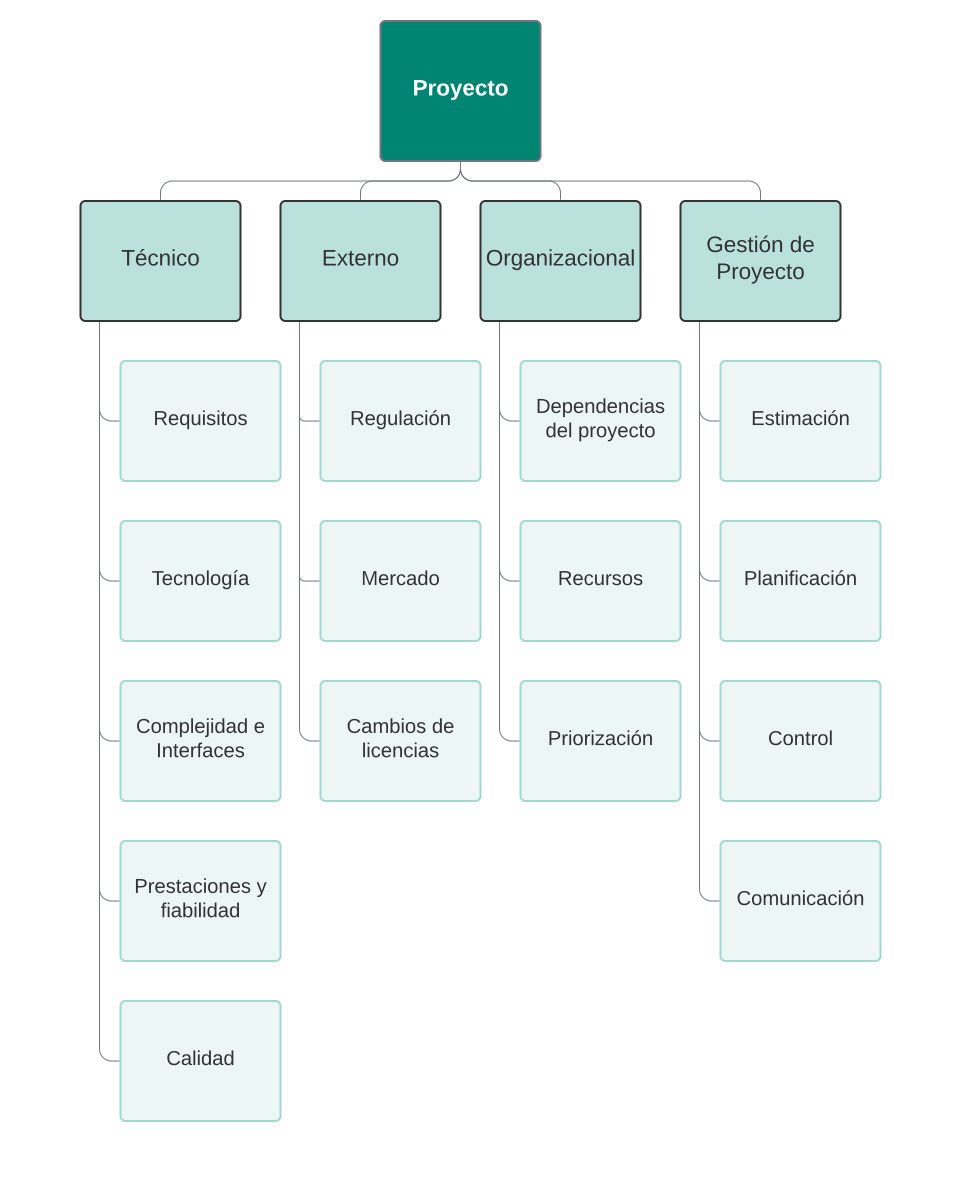
\includegraphics[width=0.65\linewidth]{figures/A1_PGR_RBS.png}
    \caption{RBS, desglose de categorías de riesgos del proyecto}
    \label{fig:A1_PGR_RBS}
\end{figure}

\subsubsection*{Probabilidad e impacto}
Para la valoración de riesgos se ha utilizado la \coloredUnderline{\hyperlink{fig:A1_PGR_matriz_prob_vs_impact}{Figura \ref*{fig:A1_PGR_matriz_prob_vs_impact}: \nameref*{fig:A1_PGR_matriz_prob_vs_impact}}} definida anteriormente. 
Esta matriz establece los valores utilizados en la priorización de riesgos. Cada riesgo tiene un valor asociado de acuerdo a su probabilidad de ocurrencia y el impacto en el proyecto.

\begin{figure}[H]
    \hypertarget{fig:A1_PGR_matriz_prob_vs_impact}{}
    \centering
    \includegraphics{figures/A1_PGR_matriz_prob_vs_impact.png}
    \caption{Matriz de probabilidad vs impacto}
    \label{fig:A1_PGR_matriz_prob_vs_impact}
\end{figure}

\subsubsection*{Identificación de riesgos}
Para la identificación de riesgos se han utilizado dos técnicas principales: la recopilación de información mediante \textit{brainstorming} y, de forma complementaria, el análisis de listas de control. La combinación de estas técnicas ha permitido una identificación de riesgos realista, abarcando tanto los riesgos inherentes al tipo de proyecto, es decir, desarrollo de software, como los riesgos específicos del proyecto en particular.

\subsubsection*{Análisis de riesgos}
Una vez identificados los riesgos, se ha procedido a analizarlos. Se ha llevado a cabo un análisis cualitativo de los riesgos que consta de los siguientes procesos:
\begin{itemize}
    \item \textbf{Evaluación de la probabilidad e impacto:} Asignación de valores de probabilidad e impacto a cada riesgo, obteniendo un valor de prioridad basado en la \coloredUnderline{\hyperlink{fig:A1_PGR_matriz_prob_vs_impact}{Figura \ref*{fig:A1_PGR_matriz_prob_vs_impact}: \nameref*{fig:A1_PGR_matriz_prob_vs_impact}}}.
    \item \textbf{Categorización de riesgos:} Clasificación de los riesgos identificados según las categorías de riesgos establecidas en  \coloredUnderline{\hyperlink{fig:A1_PGR_RBS}{Figura \ref*{fig:A1_PGR_RBS}: \nameref*{fig:A1_PGR_RBS}}}.
    \item \textbf{Evaluación de la urgencia:} Priorización preliminar de los riesgos basada en la urgencia con la que deben ser tratados.
\end{itemize}


\subsubsection*{Priorización}
Una vez analizados los riesgos, se procede a su priorización. A cada riesgo se le asigna un valor de prioridad basado en los resultados del análisis de probabilidad e impacto, así como en la evaluación de la urgencia.

De esta manera, se obtiene una lista de riesgos ordenada de mayor a menor importancia, lo que permite centrar los esfuerzos en los riesgos más críticos.

\subsubsection*{Planificación de la gestión de cada riesgo}
Se lleva a cabo un análisis más detallado de los riesgos definiendo las estrategias de respuesta a los mismos. 
En el proyecto se ha optado por las siguientes estrategias de respuesta:
\begin{itemize}
    \item \textbf{Evitar el riesgo:} Se trata de eliminar la amenaza o la oportunidad que representa el riesgo.
    \item \textbf{Transferir el riesgo:} Se trata de trasladar la responsabilidad del riesgo a un tercero.
    \item \textbf{Mitigar el riesgo:} Se trata de reducir la probabilidad de ocurrencia o en caso de que ocurra, reducir el impacto.
    \item \textbf{Aceptar el riesgo:} Se trata de asumir las consecuencias del riesgo y convivir con él.
\end{itemize}

\subsubsection*{Resolución de riesgos}
Una vez planificadas las respuestas a los riesgos, se procede a la resolución de los mismos determinando si los riesgos son eliminados o solucionados. 
Para ello se ha llevado a cabo un desarrollo incremental con el fin de minimizar los riesgos y permitir una mayor flexibilidad en la gestión de los mismos.

\subsubsection*{Monitorización y control de riesgos}
Por último, se establece un plan de monitorización y control de riesgos. 
La principal técnica utilizada para la monitorización y control de riesgos son las reuniones periódicas de seguimiento del proyecto, en las que se controla el progreso del proyecto, se revisan los riesgos y se actualiza la información de los mismos tomando las medidas correctoras necesarias en cada momento.



\newpage
\phantomsection
\addcontentsline{toc}{section}{CONTENIDO ENTREGADO EN LOS ANEXOS}
\section*{CONTENIDO ENTREGADO EN LOS ANEXOS} 
\input{Anexos/A2_Contenido_entregado}

% ----- Página de Bibliografía -----

\newpage
\nocite{*} %El comando bibliography enseña solo las referencias que se hayan usado en el texto. Este comando permite "no citar" todas y así que aparezcan.
\bibliographystyle{ieeetr} 
\bibliography{references}

\newpage





\end{document}
